\documentclass[twoside]{book}

% Packages required by doxygen
\usepackage{fixltx2e}
\usepackage{calc}
\usepackage{doxygen}
\usepackage[export]{adjustbox} % also loads graphicx
\usepackage{graphicx}
\usepackage[utf8]{inputenc}
\usepackage{makeidx}
\usepackage{multicol}
\usepackage{multirow}
\PassOptionsToPackage{warn}{textcomp}
\usepackage{textcomp}
\usepackage[nointegrals]{wasysym}
\usepackage[table]{xcolor}

% Font selection
\usepackage[T1]{fontenc}
\usepackage[scaled=.90]{helvet}
\usepackage{courier}
\usepackage{amssymb}
\usepackage{sectsty}
\renewcommand{\familydefault}{\sfdefault}
\allsectionsfont{%
  \fontseries{bc}\selectfont%
  \color{darkgray}%
}
\renewcommand{\DoxyLabelFont}{%
  \fontseries{bc}\selectfont%
  \color{darkgray}%
}
\newcommand{\+}{\discretionary{\mbox{\scriptsize$\hookleftarrow$}}{}{}}

% Page & text layout
\usepackage{geometry}
\geometry{%
  a4paper,%
  top=2.5cm,%
  bottom=2.5cm,%
  left=2.5cm,%
  right=2.5cm%
}
\tolerance=750
\hfuzz=15pt
\hbadness=750
\setlength{\emergencystretch}{15pt}
\setlength{\parindent}{0cm}
\setlength{\parskip}{3ex plus 2ex minus 2ex}
\makeatletter
\renewcommand{\paragraph}{%
  \@startsection{paragraph}{4}{0ex}{-1.0ex}{1.0ex}{%
    \normalfont\normalsize\bfseries\SS@parafont%
  }%
}
\renewcommand{\subparagraph}{%
  \@startsection{subparagraph}{5}{0ex}{-1.0ex}{1.0ex}{%
    \normalfont\normalsize\bfseries\SS@subparafont%
  }%
}
\makeatother

% Headers & footers
\usepackage{fancyhdr}
\pagestyle{fancyplain}
\fancyhead[LE]{\fancyplain{}{\bfseries\thepage}}
\fancyhead[CE]{\fancyplain{}{}}
\fancyhead[RE]{\fancyplain{}{\bfseries\leftmark}}
\fancyhead[LO]{\fancyplain{}{\bfseries\rightmark}}
\fancyhead[CO]{\fancyplain{}{}}
\fancyhead[RO]{\fancyplain{}{\bfseries\thepage}}
\fancyfoot[LE]{\fancyplain{}{}}
\fancyfoot[CE]{\fancyplain{}{}}
\fancyfoot[RE]{\fancyplain{}{\bfseries\scriptsize Generated by Doxygen }}
\fancyfoot[LO]{\fancyplain{}{\bfseries\scriptsize Generated by Doxygen }}
\fancyfoot[CO]{\fancyplain{}{}}
\fancyfoot[RO]{\fancyplain{}{}}
\renewcommand{\footrulewidth}{0.4pt}
\renewcommand{\chaptermark}[1]{%
  \markboth{#1}{}%
}
\renewcommand{\sectionmark}[1]{%
  \markright{\thesection\ #1}%
}

% Indices & bibliography
\usepackage{natbib}
\usepackage[titles]{tocloft}
\setcounter{tocdepth}{3}
\setcounter{secnumdepth}{5}
\makeindex

% Hyperlinks (required, but should be loaded last)
\usepackage{ifpdf}
\ifpdf
  \usepackage[pdftex,pagebackref=true]{hyperref}
\else
  \usepackage[ps2pdf,pagebackref=true]{hyperref}
\fi
\hypersetup{%
  colorlinks=true,%
  linkcolor=blue,%
  citecolor=blue,%
  unicode%
}

% Custom commands
\newcommand{\clearemptydoublepage}{%
  \newpage{\pagestyle{empty}\cleardoublepage}%
}

\usepackage{caption}
\captionsetup{labelsep=space,justification=centering,font={bf},singlelinecheck=off,skip=4pt,position=top}

%===== C O N T E N T S =====

\begin{document}

% Titlepage & ToC
\hypersetup{pageanchor=false,
             bookmarksnumbered=true,
             pdfencoding=unicode
            }
\pagenumbering{alph}
\begin{titlepage}
\vspace*{7cm}
\begin{center}%
{\Large My Project }\\
\vspace*{1cm}
{\large Generated by Doxygen 1.8.13}\\
\end{center}
\end{titlepage}
\clearemptydoublepage
\pagenumbering{roman}
\tableofcontents
\clearemptydoublepage
\pagenumbering{arabic}
\hypersetup{pageanchor=true}

%--- Begin generated contents ---
\chapter{5801 S20 Team3 Voting System Iteration 2 Index Page}
\label{index}\hypertarget{index}{}\hypertarget{index_intro_sec}{}\section{Introduction}\label{index_intro_sec}
The Voting System is ... 
\chapter{Hierarchical Index}
\section{Class Hierarchy}
This inheritance list is sorted roughly, but not completely, alphabetically\+:\begin{DoxyCompactList}
\item \contentsline{section}{Ballot}{\pageref{classBallot}}{}
\item \contentsline{section}{Ballot\+File\+Processor}{\pageref{classBallotFileProcessor}}{}
\item \contentsline{section}{Candidate}{\pageref{classCandidate}}{}
\begin{DoxyCompactList}
\item \contentsline{section}{S\+T\+V\+Candidate}{\pageref{classSTVCandidate}}{}
\end{DoxyCompactList}
\item \contentsline{section}{Logger}{\pageref{classLogger}}{}
\item \contentsline{section}{Plurality\+Election}{\pageref{classPluralityElection}}{}
\item \contentsline{section}{Plurality\+Election\+Record}{\pageref{classPluralityElectionRecord}}{}
\item \contentsline{section}{Result\+Display}{\pageref{classResultDisplay}}{}
\item \contentsline{section}{S\+T\+V\+Candidate\+Comparator}{\pageref{structSTVCandidateComparator}}{}
\item \contentsline{section}{S\+T\+V\+Election}{\pageref{classSTVElection}}{}
\item \contentsline{section}{S\+T\+V\+Election\+Record}{\pageref{classSTVElectionRecord}}{}
\item \contentsline{section}{Voting\+Info}{\pageref{classVotingInfo}}{}
\end{DoxyCompactList}

\chapter{Class Index}
\section{Class List}
Here are the classes, structs, unions and interfaces with brief descriptions\+:\begin{DoxyCompactList}
\item\contentsline{section}{\hyperlink{classBallot}{Ballot} \\*The main class for ballots }{\pageref{classBallot}}{}
\item\contentsline{section}{\hyperlink{classBallotFileProcessor}{Ballot\+File\+Processor} \\*The main class for processing ballot files }{\pageref{classBallotFileProcessor}}{}
\item\contentsline{section}{\hyperlink{classCandidate}{Candidate} \\*The main class for candidates }{\pageref{classCandidate}}{}
\item\contentsline{section}{\hyperlink{classLogger}{Logger} \\*Singleton \hyperlink{classLogger}{Logger} Class }{\pageref{classLogger}}{}
\item\contentsline{section}{\hyperlink{classPluralityElection}{Plurality\+Election} \\*The main class for plurality election }{\pageref{classPluralityElection}}{}
\item\contentsline{section}{\hyperlink{classPluralityElectionRecord}{Plurality\+Election\+Record} \\*The class for the plurality election records }{\pageref{classPluralityElectionRecord}}{}
\item\contentsline{section}{\hyperlink{classSTVCandidate}{S\+T\+V\+Candidate} \\*The main class for S\+TV candidates }{\pageref{classSTVCandidate}}{}
\item\contentsline{section}{\hyperlink{classSTVElection}{S\+T\+V\+Election} \\*The main class for stv election }{\pageref{classSTVElection}}{}
\item\contentsline{section}{\hyperlink{classSTVElectionRecord}{S\+T\+V\+Election\+Record} \\*The class for the S\+TV election records }{\pageref{classSTVElectionRecord}}{}
\item\contentsline{section}{\hyperlink{classVotingInfo}{Voting\+Info} \\*The main class for storing voting information }{\pageref{classVotingInfo}}{}
\end{DoxyCompactList}

\chapter{File Index}
\section{File List}
Here is a list of all documented files with brief descriptions\+:\begin{DoxyCompactList}
\item\contentsline{section}{/home/spitz123/csci5801\+\_\+s20/repo-\/\+Team3/\+Project1/src/\hyperlink{ballot_8cc}{ballot.\+cc} }{\pageref{ballot_8cc}}{}
\item\contentsline{section}{/home/spitz123/csci5801\+\_\+s20/repo-\/\+Team3/\+Project1/src/\hyperlink{ballot_8h}{ballot.\+h} }{\pageref{ballot_8h}}{}
\item\contentsline{section}{/home/spitz123/csci5801\+\_\+s20/repo-\/\+Team3/\+Project1/src/\hyperlink{ballot__file__processor_8cc}{ballot\+\_\+file\+\_\+processor.\+cc} }{\pageref{ballot__file__processor_8cc}}{}
\item\contentsline{section}{/home/spitz123/csci5801\+\_\+s20/repo-\/\+Team3/\+Project1/src/\hyperlink{ballot__file__processor_8h}{ballot\+\_\+file\+\_\+processor.\+h} }{\pageref{ballot__file__processor_8h}}{}
\item\contentsline{section}{/home/spitz123/csci5801\+\_\+s20/repo-\/\+Team3/\+Project1/src/\hyperlink{candidate_8cc}{candidate.\+cc} }{\pageref{candidate_8cc}}{}
\item\contentsline{section}{/home/spitz123/csci5801\+\_\+s20/repo-\/\+Team3/\+Project1/src/\hyperlink{candidate_8h}{candidate.\+h} }{\pageref{candidate_8h}}{}
\item\contentsline{section}{/home/spitz123/csci5801\+\_\+s20/repo-\/\+Team3/\+Project1/src/\hyperlink{logger_8h}{logger.\+h} }{\pageref{logger_8h}}{}
\item\contentsline{section}{/home/spitz123/csci5801\+\_\+s20/repo-\/\+Team3/\+Project1/src/\hyperlink{mainpage_8h}{mainpage.\+h} }{\pageref{mainpage_8h}}{}
\item\contentsline{section}{/home/spitz123/csci5801\+\_\+s20/repo-\/\+Team3/\+Project1/src/\hyperlink{plurality__election_8cc}{plurality\+\_\+election.\+cc} }{\pageref{plurality__election_8cc}}{}
\item\contentsline{section}{/home/spitz123/csci5801\+\_\+s20/repo-\/\+Team3/\+Project1/src/\hyperlink{plurality__election_8h}{plurality\+\_\+election.\+h} }{\pageref{plurality__election_8h}}{}
\item\contentsline{section}{/home/spitz123/csci5801\+\_\+s20/repo-\/\+Team3/\+Project1/src/\hyperlink{plurality__election__record_8h}{plurality\+\_\+election\+\_\+record.\+h} }{\pageref{plurality__election__record_8h}}{}
\item\contentsline{section}{/home/spitz123/csci5801\+\_\+s20/repo-\/\+Team3/\+Project1/src/\hyperlink{result__display_8h}{result\+\_\+display.\+h} }{\pageref{result__display_8h}}{}
\item\contentsline{section}{/home/spitz123/csci5801\+\_\+s20/repo-\/\+Team3/\+Project1/src/\hyperlink{stv__election_8cc}{stv\+\_\+election.\+cc} }{\pageref{stv__election_8cc}}{}
\item\contentsline{section}{/home/spitz123/csci5801\+\_\+s20/repo-\/\+Team3/\+Project1/src/\hyperlink{stv__election_8h}{stv\+\_\+election.\+h} }{\pageref{stv__election_8h}}{}
\item\contentsline{section}{/home/spitz123/csci5801\+\_\+s20/repo-\/\+Team3/\+Project1/src/\hyperlink{stv__election__record_8h}{stv\+\_\+election\+\_\+record.\+h} }{\pageref{stv__election__record_8h}}{}
\item\contentsline{section}{/home/spitz123/csci5801\+\_\+s20/repo-\/\+Team3/\+Project1/src/\hyperlink{voting__info_8cc}{voting\+\_\+info.\+cc} }{\pageref{voting__info_8cc}}{}
\item\contentsline{section}{/home/spitz123/csci5801\+\_\+s20/repo-\/\+Team3/\+Project1/src/\hyperlink{voting__info_8h}{voting\+\_\+info.\+h} }{\pageref{voting__info_8h}}{}
\item\contentsline{section}{/home/spitz123/csci5801\+\_\+s20/repo-\/\+Team3/\+Project1/src/\hyperlink{voting__system_8cc}{voting\+\_\+system.\+cc} }{\pageref{voting__system_8cc}}{}
\end{DoxyCompactList}

\chapter{Class Documentation}
\hypertarget{classBallot}{}\section{Ballot Class Reference}
\label{classBallot}\index{Ballot@{Ballot}}


The main class for ballots.  




{\ttfamily \#include $<$ballot.\+h$>$}



Collaboration diagram for Ballot\+:\nopagebreak
\begin{figure}[H]
\begin{center}
\leavevmode
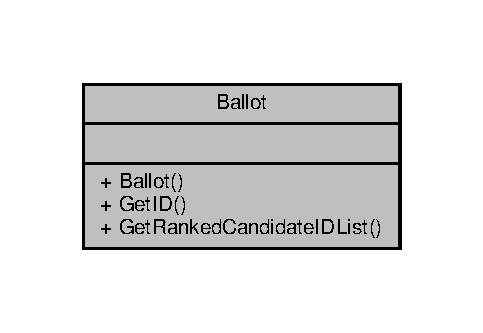
\includegraphics[width=232pt]{classBallot__coll__graph}
\end{center}
\end{figure}
\subsection*{Public Member Functions}
\begin{DoxyCompactItemize}
\item 
\hyperlink{classBallot_a890f4b9091da6f3836b5730d640869f8}{Ballot} (int, std\+::list$<$ int $>$)
\begin{DoxyCompactList}\small\item\em Constructs a ballot with a ranked candidate list and id. \end{DoxyCompactList}\item 
int \hyperlink{classBallot_ab918e416b8b0981b82b20b9df1d7ba51}{Get\+ID} ()
\begin{DoxyCompactList}\small\item\em Get ballot id. \end{DoxyCompactList}\item 
std\+::list$<$ int $>$ \hyperlink{classBallot_a5107d9df309cc5b7ff4a237799e3bff5}{Get\+Ranked\+Candidate\+I\+D\+List} ()
\begin{DoxyCompactList}\small\item\em Get the ranked candidate id list. \end{DoxyCompactList}\end{DoxyCompactItemize}


\subsection{Detailed Description}
The main class for ballots. 

Is a ballot. 

\subsection{Constructor \& Destructor Documentation}
\mbox{\Hypertarget{classBallot_a890f4b9091da6f3836b5730d640869f8}\label{classBallot_a890f4b9091da6f3836b5730d640869f8}} 
\index{Ballot@{Ballot}!Ballot@{Ballot}}
\index{Ballot@{Ballot}!Ballot@{Ballot}}
\subsubsection{\texorpdfstring{Ballot()}{Ballot()}}
{\footnotesize\ttfamily Ballot\+::\+Ballot (\begin{DoxyParamCaption}\item[{int}]{ballot\+\_\+id,  }\item[{std\+::list$<$ int $>$}]{Candidate\+List }\end{DoxyParamCaption})\hspace{0.3cm}{\ttfamily [explicit]}}



Constructs a ballot with a ranked candidate list and id. 


\begin{DoxyParams}[1]{Parameters}
\mbox{\tt in}  & {\em int} & holding a ballot id number \\
\hline
\mbox{\tt in}  & {\em linked} & list containing candidate id numbers \\
\hline
\end{DoxyParams}


\subsection{Member Function Documentation}
\mbox{\Hypertarget{classBallot_ab918e416b8b0981b82b20b9df1d7ba51}\label{classBallot_ab918e416b8b0981b82b20b9df1d7ba51}} 
\index{Ballot@{Ballot}!Get\+ID@{Get\+ID}}
\index{Get\+ID@{Get\+ID}!Ballot@{Ballot}}
\subsubsection{\texorpdfstring{Get\+I\+D()}{GetID()}}
{\footnotesize\ttfamily int Ballot\+::\+Get\+ID (\begin{DoxyParamCaption}{ }\end{DoxyParamCaption})}



Get ballot id. 

\begin{DoxyReturn}{Returns}
ballot id 
\end{DoxyReturn}
\mbox{\Hypertarget{classBallot_a5107d9df309cc5b7ff4a237799e3bff5}\label{classBallot_a5107d9df309cc5b7ff4a237799e3bff5}} 
\index{Ballot@{Ballot}!Get\+Ranked\+Candidate\+I\+D\+List@{Get\+Ranked\+Candidate\+I\+D\+List}}
\index{Get\+Ranked\+Candidate\+I\+D\+List@{Get\+Ranked\+Candidate\+I\+D\+List}!Ballot@{Ballot}}
\subsubsection{\texorpdfstring{Get\+Ranked\+Candidate\+I\+D\+List()}{GetRankedCandidateIDList()}}
{\footnotesize\ttfamily std\+::list$<$ int $>$ Ballot\+::\+Get\+Ranked\+Candidate\+I\+D\+List (\begin{DoxyParamCaption}{ }\end{DoxyParamCaption})}



Get the ranked candidate id list. 

\begin{DoxyReturn}{Returns}
std\+::list$<$int$>$ ranked candidate ID List 
\end{DoxyReturn}


The documentation for this class was generated from the following files\+:\begin{DoxyCompactItemize}
\item 
/home/spitz123/csci5801\+\_\+s20/repo-\/\+Team3/\+Project1/src/\hyperlink{ballot_8h}{ballot.\+h}\item 
/home/spitz123/csci5801\+\_\+s20/repo-\/\+Team3/\+Project1/src/\hyperlink{ballot_8cc}{ballot.\+cc}\end{DoxyCompactItemize}

\hypertarget{classBallotFileProcessor}{}\section{Ballot\+File\+Processor Class Reference}
\label{classBallotFileProcessor}\index{Ballot\+File\+Processor@{Ballot\+File\+Processor}}


The main class for processing ballot files.  




{\ttfamily \#include $<$ballot\+\_\+file\+\_\+processor.\+h$>$}



Collaboration diagram for Ballot\+File\+Processor\+:\nopagebreak
\begin{figure}[H]
\begin{center}
\leavevmode
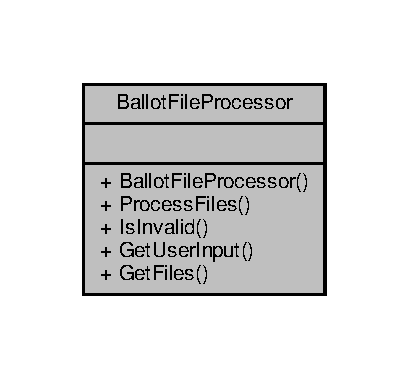
\includegraphics[width=202pt]{classBallotFileProcessor__coll__graph}
\end{center}
\end{figure}
\subsection*{Public Member Functions}
\begin{DoxyCompactItemize}
\item 
\hyperlink{classBallotFileProcessor_aadc47aedf9172bfc26b2b6324dc40576}{Ballot\+File\+Processor} (std\+::string=\char`\"{}\char`\"{})
\begin{DoxyCompactList}\small\item\em Constructs a ballot file processor with standard empty string. \end{DoxyCompactList}\item 
\mbox{\Hypertarget{classBallotFileProcessor_a372429408537c8919b969a23c3cc7e41}\label{classBallotFileProcessor_a372429408537c8919b969a23c3cc7e41}} 
\hyperlink{classBallotFileProcessor_a372429408537c8919b969a23c3cc7e41}{$\sim$\+Ballot\+File\+Processor} ()
\begin{DoxyCompactList}\small\item\em Deconstructs a ballot file processor. \end{DoxyCompactList}\item 
void \hyperlink{classBallotFileProcessor_a3d25f1db840f21ab7d19f4b4898193c9}{Process\+Files} (\hyperlink{classVotingInfo}{Voting\+Info} $\ast$)
\begin{DoxyCompactList}\small\item\em Processes ballot files. \end{DoxyCompactList}\end{DoxyCompactItemize}


\subsection{Detailed Description}
The main class for processing ballot files. 

Is a ballot file processor. 

\subsection{Constructor \& Destructor Documentation}
\mbox{\Hypertarget{classBallotFileProcessor_aadc47aedf9172bfc26b2b6324dc40576}\label{classBallotFileProcessor_aadc47aedf9172bfc26b2b6324dc40576}} 
\index{Ballot\+File\+Processor@{Ballot\+File\+Processor}!Ballot\+File\+Processor@{Ballot\+File\+Processor}}
\index{Ballot\+File\+Processor@{Ballot\+File\+Processor}!Ballot\+File\+Processor@{Ballot\+File\+Processor}}
\subsubsection{\texorpdfstring{Ballot\+File\+Processor()}{BallotFileProcessor()}}
{\footnotesize\ttfamily Ballot\+File\+Processor\+::\+Ballot\+File\+Processor (\begin{DoxyParamCaption}\item[{std\+::string}]{ballotfilename = {\ttfamily \char`\"{}\char`\"{}} }\end{DoxyParamCaption})\hspace{0.3cm}{\ttfamily [explicit]}}



Constructs a ballot file processor with standard empty string. 


\begin{DoxyParams}[1]{Parameters}
\mbox{\tt in}  & {\em string} & holding text of a csv ballot file. \\
\hline
\end{DoxyParams}


\subsection{Member Function Documentation}
\mbox{\Hypertarget{classBallotFileProcessor_a3d25f1db840f21ab7d19f4b4898193c9}\label{classBallotFileProcessor_a3d25f1db840f21ab7d19f4b4898193c9}} 
\index{Ballot\+File\+Processor@{Ballot\+File\+Processor}!Process\+Files@{Process\+Files}}
\index{Process\+Files@{Process\+Files}!Ballot\+File\+Processor@{Ballot\+File\+Processor}}
\subsubsection{\texorpdfstring{Process\+Files()}{ProcessFiles()}}
{\footnotesize\ttfamily void Ballot\+File\+Processor\+::\+Process\+Files (\begin{DoxyParamCaption}\item[{\hyperlink{classVotingInfo}{Voting\+Info} $\ast$}]{votinginfo }\end{DoxyParamCaption})}



Processes ballot files. 


\begin{DoxyParams}[1]{Parameters}
\mbox{\tt in}  & {\em pointer} & to \hyperlink{classVotingInfo}{Voting\+Info} object with algorithm and seat info. \\
\hline
\end{DoxyParams}


The documentation for this class was generated from the following files\+:\begin{DoxyCompactItemize}
\item 
/home/spitz123/csci5801\+\_\+s20/repo-\/\+Team3/\+Project1/src/\hyperlink{ballot__file__processor_8h}{ballot\+\_\+file\+\_\+processor.\+h}\item 
/home/spitz123/csci5801\+\_\+s20/repo-\/\+Team3/\+Project1/src/\hyperlink{ballot__file__processor_8cc}{ballot\+\_\+file\+\_\+processor.\+cc}\end{DoxyCompactItemize}

\hypertarget{classCandidate}{}\section{Candidate Class Reference}
\label{classCandidate}\index{Candidate@{Candidate}}


The main class for candidates.  




{\ttfamily \#include $<$candidate.\+h$>$}



Inheritance diagram for Candidate\+:\nopagebreak
\begin{figure}[H]
\begin{center}
\leavevmode
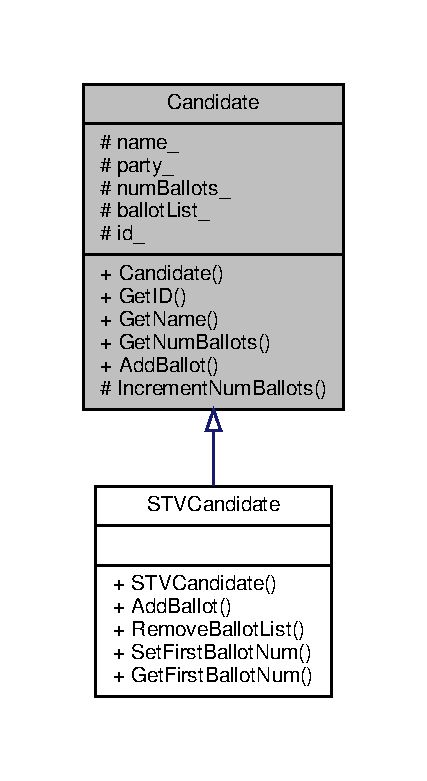
\includegraphics[width=205pt]{classCandidate__inherit__graph}
\end{center}
\end{figure}


Collaboration diagram for Candidate\+:\nopagebreak
\begin{figure}[H]
\begin{center}
\leavevmode
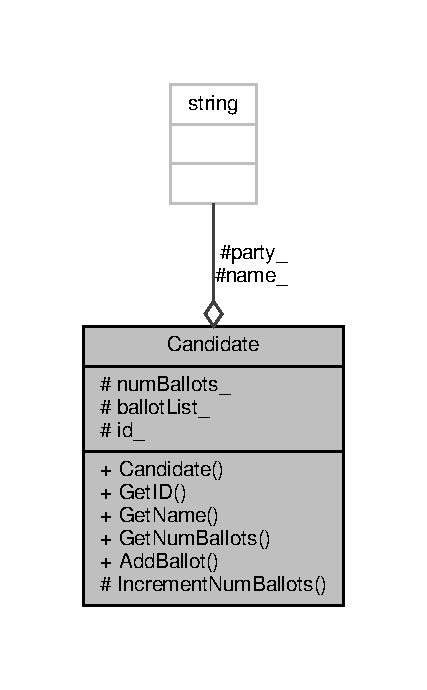
\includegraphics[width=205pt]{classCandidate__coll__graph}
\end{center}
\end{figure}
\subsection*{Public Member Functions}
\begin{DoxyCompactItemize}
\item 
\hyperlink{classCandidate_a5687946f621baf578fe2391272481dc5}{Candidate} (int, std\+::string, std\+::string)
\begin{DoxyCompactList}\small\item\em Constructs a candidate to be used in an election. \end{DoxyCompactList}\item 
int \hyperlink{classCandidate_a29b844b51162c153c6f85cf817c1c9d2}{Get\+ID} () const
\begin{DoxyCompactList}\small\item\em Get candidate id. \end{DoxyCompactList}\item 
std\+::string \hyperlink{classCandidate_ad1ca1432a295579d2d61fd50a5988973}{Get\+Name} () const
\begin{DoxyCompactList}\small\item\em Get the candidate\textquotesingle{}s name. \end{DoxyCompactList}\item 
int \hyperlink{classCandidate_a966911d3f565a2d31cf9780b522340d8}{Get\+Num\+Ballots} () const
\begin{DoxyCompactList}\small\item\em Get the number of ballots the candidate has. \end{DoxyCompactList}\item 
int \hyperlink{classCandidate_af33985d301d94d4855d28b891aba1ed6}{Add\+Ballot} (\hyperlink{classBallot}{Ballot} $\ast$)
\begin{DoxyCompactList}\small\item\em Add a ballot to the list of ballots the candidate has. \end{DoxyCompactList}\end{DoxyCompactItemize}
\subsection*{Protected Member Functions}
\begin{DoxyCompactItemize}
\item 
int \hyperlink{classCandidate_a15a55468662174c8189b32fe344deb9e}{Increment\+Num\+Ballots} ()
\begin{DoxyCompactList}\small\item\em Add one to the number of ballots the candidate has. \end{DoxyCompactList}\end{DoxyCompactItemize}
\subsection*{Protected Attributes}
\begin{DoxyCompactItemize}
\item 
\mbox{\Hypertarget{classCandidate_a70cca9349b891eb921bfdeabe7ded6d5}\label{classCandidate_a70cca9349b891eb921bfdeabe7ded6d5}} 
std\+::string {\bfseries name\+\_\+}
\item 
\mbox{\Hypertarget{classCandidate_a0bfc84bce32a43270d2387aea8ce2cdf}\label{classCandidate_a0bfc84bce32a43270d2387aea8ce2cdf}} 
std\+::string {\bfseries party\+\_\+}
\item 
\mbox{\Hypertarget{classCandidate_aec8aa8cbbd790386924e7b57b84c9081}\label{classCandidate_aec8aa8cbbd790386924e7b57b84c9081}} 
int {\bfseries num\+Ballots\+\_\+} = 0
\item 
\mbox{\Hypertarget{classCandidate_ab1454bc82abc3f3b417bdf81de09fc0c}\label{classCandidate_ab1454bc82abc3f3b417bdf81de09fc0c}} 
std\+::list$<$ \hyperlink{classBallot}{Ballot} $\ast$ $>$ {\bfseries ballot\+List\+\_\+} = \{\}
\item 
\mbox{\Hypertarget{classCandidate_a04149c9b00ec326c2d81cc607c29271c}\label{classCandidate_a04149c9b00ec326c2d81cc607c29271c}} 
int {\bfseries id\+\_\+}
\end{DoxyCompactItemize}


\subsection{Detailed Description}
The main class for candidates. 

Is a candidate. 

\subsection{Constructor \& Destructor Documentation}
\mbox{\Hypertarget{classCandidate_a5687946f621baf578fe2391272481dc5}\label{classCandidate_a5687946f621baf578fe2391272481dc5}} 
\index{Candidate@{Candidate}!Candidate@{Candidate}}
\index{Candidate@{Candidate}!Candidate@{Candidate}}
\subsubsection{\texorpdfstring{Candidate()}{Candidate()}}
{\footnotesize\ttfamily Candidate\+::\+Candidate (\begin{DoxyParamCaption}\item[{int}]{candidate\+\_\+num = {\ttfamily 0},  }\item[{std\+::string}]{candidate\+\_\+name = {\ttfamily \char`\"{}\char`\"{}},  }\item[{std\+::string}]{candidate\+\_\+party = {\ttfamily \char`\"{}\char`\"{}} }\end{DoxyParamCaption})\hspace{0.3cm}{\ttfamily [explicit]}}



Constructs a candidate to be used in an election. 


\begin{DoxyParams}[1]{Parameters}
\mbox{\tt in}  & {\em int} & holding a candidate id number \\
\hline
\mbox{\tt in}  & {\em string} & containing the candidate\textquotesingle{}s name \\
\hline
\mbox{\tt in}  & {\em string} & containing the candidate\textquotesingle{}s party \\
\hline
\end{DoxyParams}


\subsection{Member Function Documentation}
\mbox{\Hypertarget{classCandidate_af33985d301d94d4855d28b891aba1ed6}\label{classCandidate_af33985d301d94d4855d28b891aba1ed6}} 
\index{Candidate@{Candidate}!Add\+Ballot@{Add\+Ballot}}
\index{Add\+Ballot@{Add\+Ballot}!Candidate@{Candidate}}
\subsubsection{\texorpdfstring{Add\+Ballot()}{AddBallot()}}
{\footnotesize\ttfamily int Candidate\+::\+Add\+Ballot (\begin{DoxyParamCaption}\item[{\hyperlink{classBallot}{Ballot} $\ast$}]{ballot }\end{DoxyParamCaption})}



Add a ballot to the list of ballots the candidate has. 


\begin{DoxyParams}[1]{Parameters}
\mbox{\tt in}  & {\em A} & ballot object \\
\hline
\end{DoxyParams}
\begin{DoxyReturn}{Returns}
int of the number of ballots the candidate has 
\end{DoxyReturn}
\mbox{\Hypertarget{classCandidate_a29b844b51162c153c6f85cf817c1c9d2}\label{classCandidate_a29b844b51162c153c6f85cf817c1c9d2}} 
\index{Candidate@{Candidate}!Get\+ID@{Get\+ID}}
\index{Get\+ID@{Get\+ID}!Candidate@{Candidate}}
\subsubsection{\texorpdfstring{Get\+I\+D()}{GetID()}}
{\footnotesize\ttfamily int Candidate\+::\+Get\+ID (\begin{DoxyParamCaption}{ }\end{DoxyParamCaption}) const}



Get candidate id. 

\begin{DoxyReturn}{Returns}
candidate id 
\end{DoxyReturn}
\mbox{\Hypertarget{classCandidate_ad1ca1432a295579d2d61fd50a5988973}\label{classCandidate_ad1ca1432a295579d2d61fd50a5988973}} 
\index{Candidate@{Candidate}!Get\+Name@{Get\+Name}}
\index{Get\+Name@{Get\+Name}!Candidate@{Candidate}}
\subsubsection{\texorpdfstring{Get\+Name()}{GetName()}}
{\footnotesize\ttfamily std\+::string Candidate\+::\+Get\+Name (\begin{DoxyParamCaption}{ }\end{DoxyParamCaption}) const}



Get the candidate\textquotesingle{}s name. 

\begin{DoxyReturn}{Returns}
string of the candidate\textquotesingle{}s name 
\end{DoxyReturn}
\mbox{\Hypertarget{classCandidate_a966911d3f565a2d31cf9780b522340d8}\label{classCandidate_a966911d3f565a2d31cf9780b522340d8}} 
\index{Candidate@{Candidate}!Get\+Num\+Ballots@{Get\+Num\+Ballots}}
\index{Get\+Num\+Ballots@{Get\+Num\+Ballots}!Candidate@{Candidate}}
\subsubsection{\texorpdfstring{Get\+Num\+Ballots()}{GetNumBallots()}}
{\footnotesize\ttfamily int Candidate\+::\+Get\+Num\+Ballots (\begin{DoxyParamCaption}{ }\end{DoxyParamCaption}) const}



Get the number of ballots the candidate has. 

\begin{DoxyReturn}{Returns}
int of the number of ballots the candidate has 
\end{DoxyReturn}
\mbox{\Hypertarget{classCandidate_a15a55468662174c8189b32fe344deb9e}\label{classCandidate_a15a55468662174c8189b32fe344deb9e}} 
\index{Candidate@{Candidate}!Increment\+Num\+Ballots@{Increment\+Num\+Ballots}}
\index{Increment\+Num\+Ballots@{Increment\+Num\+Ballots}!Candidate@{Candidate}}
\subsubsection{\texorpdfstring{Increment\+Num\+Ballots()}{IncrementNumBallots()}}
{\footnotesize\ttfamily int Candidate\+::\+Increment\+Num\+Ballots (\begin{DoxyParamCaption}{ }\end{DoxyParamCaption})\hspace{0.3cm}{\ttfamily [protected]}}



Add one to the number of ballots the candidate has. 

\begin{DoxyReturn}{Returns}
int of the number of ballots the candidate has 
\end{DoxyReturn}


The documentation for this class was generated from the following files\+:\begin{DoxyCompactItemize}
\item 
/home/spitz123/csci5801\+\_\+s20/repo-\/\+Team3/\+Project1/src/\hyperlink{candidate_8h}{candidate.\+h}\item 
/home/spitz123/csci5801\+\_\+s20/repo-\/\+Team3/\+Project1/src/\hyperlink{candidate_8cc}{candidate.\+cc}\end{DoxyCompactItemize}

\hypertarget{classLogger}{}\section{Logger Class Reference}
\label{classLogger}\index{Logger@{Logger}}


The main class for logging info to an audit file.  




{\ttfamily \#include $<$logger.\+h$>$}



Collaboration diagram for Logger\+:\nopagebreak
\begin{figure}[H]
\begin{center}
\leavevmode
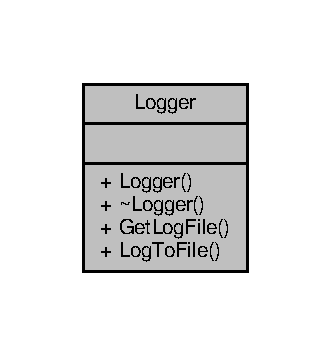
\includegraphics[width=159pt]{classLogger__coll__graph}
\end{center}
\end{figure}
\subsection*{Public Member Functions}
\begin{DoxyCompactItemize}
\item 
\hyperlink{classLogger_abc41bfb031d896170c7675fa96a6b30c}{Logger} ()
\begin{DoxyCompactList}\small\item\em Constructs an object to use to log election information to a file. \end{DoxyCompactList}\item 
\mbox{\Hypertarget{classLogger_acb668a9e186a25fbaad2e4af6d1ed00a}\label{classLogger_acb668a9e186a25fbaad2e4af6d1ed00a}} 
\hyperlink{classLogger_acb668a9e186a25fbaad2e4af6d1ed00a}{$\sim$\+Logger} ()
\begin{DoxyCompactList}\small\item\em Deconstructs election logging object. \end{DoxyCompactList}\item 
\mbox{\Hypertarget{classLogger_ad22a485469cc14c5266e5fda019aba4d}\label{classLogger_ad22a485469cc14c5266e5fda019aba4d}} 
std\+::string \hyperlink{classLogger_ad22a485469cc14c5266e5fda019aba4d}{Get\+Log\+File} ()
\begin{DoxyCompactList}\small\item\em Get the file name of the election information audit file. \end{DoxyCompactList}\item 
void \hyperlink{classLogger_adb535266f5ad2a27ce2bd589884f347b}{Log\+To\+File} (std\+::string message)
\begin{DoxyCompactList}\small\item\em Send a message to the logger to append to an election information file. \end{DoxyCompactList}\end{DoxyCompactItemize}


\subsection{Detailed Description}
The main class for logging info to an audit file. 

Is an election file logger 

\subsection{Constructor \& Destructor Documentation}
\mbox{\Hypertarget{classLogger_abc41bfb031d896170c7675fa96a6b30c}\label{classLogger_abc41bfb031d896170c7675fa96a6b30c}} 
\index{Logger@{Logger}!Logger@{Logger}}
\index{Logger@{Logger}!Logger@{Logger}}
\subsubsection{\texorpdfstring{Logger()}{Logger()}}
{\footnotesize\ttfamily Logger\+::\+Logger (\begin{DoxyParamCaption}{ }\end{DoxyParamCaption})}



Constructs an object to use to log election information to a file. 


\begin{DoxyParams}[1]{Parameters}
\mbox{\tt in}  & {\em string} & holding text of a csv ballot file. \\
\hline
\end{DoxyParams}


\subsection{Member Function Documentation}
\mbox{\Hypertarget{classLogger_adb535266f5ad2a27ce2bd589884f347b}\label{classLogger_adb535266f5ad2a27ce2bd589884f347b}} 
\index{Logger@{Logger}!Log\+To\+File@{Log\+To\+File}}
\index{Log\+To\+File@{Log\+To\+File}!Logger@{Logger}}
\subsubsection{\texorpdfstring{Log\+To\+File()}{LogToFile()}}
{\footnotesize\ttfamily void Logger\+::\+Log\+To\+File (\begin{DoxyParamCaption}\item[{std\+::string}]{message }\end{DoxyParamCaption})}



Send a message to the logger to append to an election information file. 


\begin{DoxyParams}[1]{Parameters}
\mbox{\tt in}  & {\em message} & to be written to the election information file. \\
\hline
\end{DoxyParams}


The documentation for this class was generated from the following files\+:\begin{DoxyCompactItemize}
\item 
/home/spitz123/csci5801\+\_\+s20/repo-\/\+Team3/\+Project1/src/\hyperlink{logger_8h}{logger.\+h}\item 
/home/spitz123/csci5801\+\_\+s20/repo-\/\+Team3/\+Project1/src/logger.\+cc\end{DoxyCompactItemize}

\hypertarget{classPluralityElection}{}\section{Plurality\+Election Class Reference}
\label{classPluralityElection}\index{Plurality\+Election@{Plurality\+Election}}


The main class for plurality election.  




{\ttfamily \#include $<$plurality\+\_\+election.\+h$>$}



Collaboration diagram for Plurality\+Election\+:\nopagebreak
\begin{figure}[H]
\begin{center}
\leavevmode
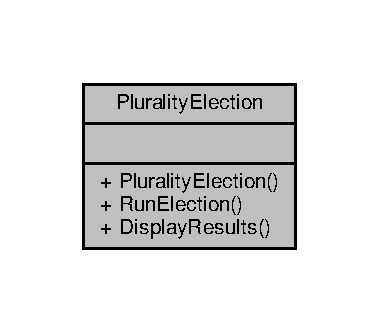
\includegraphics[width=182pt]{classPluralityElection__coll__graph}
\end{center}
\end{figure}
\subsection*{Public Member Functions}
\begin{DoxyCompactItemize}
\item 
\mbox{\Hypertarget{classPluralityElection_a9def74d2543d2c9cd71ef5f18a379dc6}\label{classPluralityElection_a9def74d2543d2c9cd71ef5f18a379dc6}} 
\hyperlink{classPluralityElection_a9def74d2543d2c9cd71ef5f18a379dc6}{Plurality\+Election} ()
\begin{DoxyCompactList}\small\item\em Constructs an \hyperlink{classPluralityElection}{Plurality\+Election} object to be used in an election. \end{DoxyCompactList}\item 
void \hyperlink{classPluralityElection_aef5d1b066923d289571e49cc5d9836e7}{Run\+Election} (\hyperlink{classVotingInfo}{Voting\+Info} $\ast$)
\begin{DoxyCompactList}\small\item\em Run a plurality election. \end{DoxyCompactList}\item 
void \hyperlink{classPluralityElection_a7e2e3eb5e4ccdff5f9f57a7a17148608}{Display\+Results} (\hyperlink{classPluralityElectionRecord}{Plurality\+Election\+Record} $\ast$, \hyperlink{classVotingInfo}{Voting\+Info} $\ast$)
\begin{DoxyCompactList}\small\item\em Print plurality election results. \end{DoxyCompactList}\end{DoxyCompactItemize}


\subsection{Detailed Description}
The main class for plurality election. 

Is an plurality election. 

\subsection{Member Function Documentation}
\mbox{\Hypertarget{classPluralityElection_a7e2e3eb5e4ccdff5f9f57a7a17148608}\label{classPluralityElection_a7e2e3eb5e4ccdff5f9f57a7a17148608}} 
\index{Plurality\+Election@{Plurality\+Election}!Display\+Results@{Display\+Results}}
\index{Display\+Results@{Display\+Results}!Plurality\+Election@{Plurality\+Election}}
\subsubsection{\texorpdfstring{Display\+Results()}{DisplayResults()}}
{\footnotesize\ttfamily void Plurality\+Election\+::\+Display\+Results (\begin{DoxyParamCaption}\item[{\hyperlink{classPluralityElectionRecord}{Plurality\+Election\+Record} $\ast$}]{election\+\_\+record,  }\item[{\hyperlink{classVotingInfo}{Voting\+Info} $\ast$}]{voting\+\_\+info }\end{DoxyParamCaption})}



Print plurality election results. 


\begin{DoxyParams}[1]{Parameters}
\mbox{\tt in}  & {\em Plurality\+Election\+Record$\ast$,pointer} & to an election record. \\
\hline
\mbox{\tt in}  & {\em Voting\+Info$\ast$,a} & pointer to a \hyperlink{classVotingInfo}{Voting\+Info} object \\
\hline
\end{DoxyParams}
\begin{DoxyReturn}{Returns}
void 
\end{DoxyReturn}
\mbox{\Hypertarget{classPluralityElection_aef5d1b066923d289571e49cc5d9836e7}\label{classPluralityElection_aef5d1b066923d289571e49cc5d9836e7}} 
\index{Plurality\+Election@{Plurality\+Election}!Run\+Election@{Run\+Election}}
\index{Run\+Election@{Run\+Election}!Plurality\+Election@{Plurality\+Election}}
\subsubsection{\texorpdfstring{Run\+Election()}{RunElection()}}
{\footnotesize\ttfamily void Plurality\+Election\+::\+Run\+Election (\begin{DoxyParamCaption}\item[{\hyperlink{classVotingInfo}{Voting\+Info} $\ast$}]{voting\+Info }\end{DoxyParamCaption})}



Run a plurality election. 


\begin{DoxyParams}[1]{Parameters}
\mbox{\tt in}  & {\em Voting\+Info$\ast$,a} & pointer to a \hyperlink{classVotingInfo}{Voting\+Info} object \\
\hline
\end{DoxyParams}
\begin{DoxyReturn}{Returns}
void 
\end{DoxyReturn}


The documentation for this class was generated from the following files\+:\begin{DoxyCompactItemize}
\item 
/home/spitz123/csci5801\+\_\+s20/repo-\/\+Team3/\+Project2/src/\hyperlink{plurality__election_8h}{plurality\+\_\+election.\+h}\item 
/home/spitz123/csci5801\+\_\+s20/repo-\/\+Team3/\+Project2/src/\hyperlink{plurality__election_8cc}{plurality\+\_\+election.\+cc}\end{DoxyCompactItemize}

\hypertarget{classPluralityElectionRecord}{}\section{Plurality\+Election\+Record Class Reference}
\label{classPluralityElectionRecord}\index{Plurality\+Election\+Record@{Plurality\+Election\+Record}}


The class for the plurality election records.  




{\ttfamily \#include $<$plurality\+\_\+election\+\_\+record.\+h$>$}



Collaboration diagram for Plurality\+Election\+Record\+:\nopagebreak
\begin{figure}[H]
\begin{center}
\leavevmode
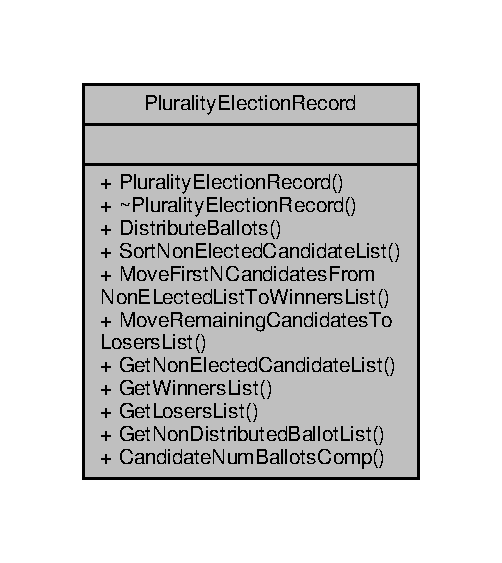
\includegraphics[width=241pt]{classPluralityElectionRecord__coll__graph}
\end{center}
\end{figure}
\subsection*{Public Member Functions}
\begin{DoxyCompactItemize}
\item 
\hyperlink{classPluralityElectionRecord_a6cc4b921ebfed3f5003b3047fae68fc5}{Plurality\+Election\+Record} (std\+::list$<$ \hyperlink{classCandidate}{Candidate} $\ast$$>$, std\+::list$<$ \hyperlink{classBallot}{Ballot} $\ast$$>$)
\begin{DoxyCompactList}\small\item\em Constructs plurality election record with a list of candidates and list of ballots. \end{DoxyCompactList}\item 
\mbox{\Hypertarget{classPluralityElectionRecord_ae04ff63f885d88bb3160621802855413}\label{classPluralityElectionRecord_ae04ff63f885d88bb3160621802855413}} 
\hyperlink{classPluralityElectionRecord_ae04ff63f885d88bb3160621802855413}{$\sim$\+Plurality\+Election\+Record} ()
\begin{DoxyCompactList}\small\item\em Deconstructs a Plurality election record container. \end{DoxyCompactList}\item 
\mbox{\Hypertarget{classPluralityElectionRecord_a0429e5fd83d0583d0077c51b163cae23}\label{classPluralityElectionRecord_a0429e5fd83d0583d0077c51b163cae23}} 
void \hyperlink{classPluralityElectionRecord_a0429e5fd83d0583d0077c51b163cae23}{Distribute\+Ballots} ()
\begin{DoxyCompactList}\small\item\em Distributes ballots to candidates. \end{DoxyCompactList}\item 
\mbox{\Hypertarget{classPluralityElectionRecord_a922a4048844b20b6eb5702abc7c99b97}\label{classPluralityElectionRecord_a922a4048844b20b6eb5702abc7c99b97}} 
void \hyperlink{classPluralityElectionRecord_a922a4048844b20b6eb5702abc7c99b97}{Sort\+Non\+Elected\+Candidate\+List} ()
\begin{DoxyCompactList}\small\item\em Sorts the non\+Elected\+Candidate\+List, candidate with the highest number of ballots is sent to front of the list. \end{DoxyCompactList}\item 
void \hyperlink{classPluralityElectionRecord_a9463aecae88c5decfdbb793678b16c87}{Move\+First\+N\+Candidates\+From\+Non\+E\+Lected\+List\+To\+Winners\+List} (int)
\begin{DoxyCompactList}\small\item\em Moves Candidates from the non elected candidate list to the winners list. \end{DoxyCompactList}\item 
\mbox{\Hypertarget{classPluralityElectionRecord_aed6bc13b7af6b3747f0bfde6d19d47b4}\label{classPluralityElectionRecord_aed6bc13b7af6b3747f0bfde6d19d47b4}} 
void \hyperlink{classPluralityElectionRecord_aed6bc13b7af6b3747f0bfde6d19d47b4}{Move\+Remaining\+Candidates\+To\+Losers\+List} ()
\begin{DoxyCompactList}\small\item\em Moves Candidates from the non elected candidate list to the losers list. \end{DoxyCompactList}\item 
std\+::list$<$ \hyperlink{classCandidate}{Candidate} $\ast$ $>$ \hyperlink{classPluralityElectionRecord_a3767192b33477411922f21ef4474f2e5}{Get\+Non\+Elected\+Candidate\+List} ()
\begin{DoxyCompactList}\small\item\em Gets the candidates that are not on the winners list or losers list. \end{DoxyCompactList}\item 
std\+::list$<$ \hyperlink{classCandidate}{Candidate} $\ast$ $>$ \hyperlink{classPluralityElectionRecord_a5b5da69173023ac0441918b0485b58b9}{Get\+Winners\+List} ()
\begin{DoxyCompactList}\small\item\em Gets the candidates that are on the winners list. \end{DoxyCompactList}\item 
std\+::list$<$ \hyperlink{classCandidate}{Candidate} $\ast$ $>$ \hyperlink{classPluralityElectionRecord_af998fcfa909f9e781ab5c48bd6b54d77}{Get\+Losers\+List} ()
\begin{DoxyCompactList}\small\item\em Gets the candidates that are on the losers list. \end{DoxyCompactList}\item 
std\+::list$<$ \hyperlink{classBallot}{Ballot} $\ast$ $>$ \hyperlink{classPluralityElectionRecord_a996f0e14812b0b1d510af52ab0c496bf}{Get\+Non\+Distributed\+Ballot\+List} ()
\begin{DoxyCompactList}\small\item\em Gets the list of ballots that haven\textquotesingle{}t yet been assigned to a candidate. \end{DoxyCompactList}\end{DoxyCompactItemize}
\subsection*{Static Public Member Functions}
\begin{DoxyCompactItemize}
\item 
static bool \hyperlink{classPluralityElectionRecord_af7b9fef847ef615ff844912a1a851a62}{Candidate\+Num\+Ballots\+Comp} (\hyperlink{classCandidate}{Candidate} $\ast$, \hyperlink{classCandidate}{Candidate} $\ast$)
\begin{DoxyCompactList}\small\item\em Moves Candidates from the non elected candidate list to the losers list. \end{DoxyCompactList}\end{DoxyCompactItemize}


\subsection{Detailed Description}
The class for the plurality election records. 

Is a Plurality Election Record -\/ will do most of plurality election work. 

\subsection{Constructor \& Destructor Documentation}
\mbox{\Hypertarget{classPluralityElectionRecord_a6cc4b921ebfed3f5003b3047fae68fc5}\label{classPluralityElectionRecord_a6cc4b921ebfed3f5003b3047fae68fc5}} 
\index{Plurality\+Election\+Record@{Plurality\+Election\+Record}!Plurality\+Election\+Record@{Plurality\+Election\+Record}}
\index{Plurality\+Election\+Record@{Plurality\+Election\+Record}!Plurality\+Election\+Record@{Plurality\+Election\+Record}}
\subsubsection{\texorpdfstring{Plurality\+Election\+Record()}{PluralityElectionRecord()}}
{\footnotesize\ttfamily Plurality\+Election\+Record\+::\+Plurality\+Election\+Record (\begin{DoxyParamCaption}\item[{std\+::list$<$ \hyperlink{classCandidate}{Candidate} $\ast$$>$}]{candidates,  }\item[{std\+::list$<$ \hyperlink{classBallot}{Ballot} $\ast$$>$}]{ballots }\end{DoxyParamCaption})\hspace{0.3cm}{\ttfamily [explicit]}}



Constructs plurality election record with a list of candidates and list of ballots. 


\begin{DoxyParams}[1]{Parameters}
\mbox{\tt in}  & {\em } & \\
\hline
\end{DoxyParams}


\subsection{Member Function Documentation}
\mbox{\Hypertarget{classPluralityElectionRecord_af7b9fef847ef615ff844912a1a851a62}\label{classPluralityElectionRecord_af7b9fef847ef615ff844912a1a851a62}} 
\index{Plurality\+Election\+Record@{Plurality\+Election\+Record}!Candidate\+Num\+Ballots\+Comp@{Candidate\+Num\+Ballots\+Comp}}
\index{Candidate\+Num\+Ballots\+Comp@{Candidate\+Num\+Ballots\+Comp}!Plurality\+Election\+Record@{Plurality\+Election\+Record}}
\subsubsection{\texorpdfstring{Candidate\+Num\+Ballots\+Comp()}{CandidateNumBallotsComp()}}
{\footnotesize\ttfamily bool Plurality\+Election\+Record\+::\+Candidate\+Num\+Ballots\+Comp (\begin{DoxyParamCaption}\item[{\hyperlink{classCandidate}{Candidate} $\ast$}]{candidate1,  }\item[{\hyperlink{classCandidate}{Candidate} $\ast$}]{candidate2 }\end{DoxyParamCaption})\hspace{0.3cm}{\ttfamily [static]}}



Moves Candidates from the non elected candidate list to the losers list. 


\begin{DoxyParams}[1]{Parameters}
\mbox{\tt in}  & {\em int} & Number of candidates to move to the losers list \\
\hline
\end{DoxyParams}
\mbox{\Hypertarget{classPluralityElectionRecord_af998fcfa909f9e781ab5c48bd6b54d77}\label{classPluralityElectionRecord_af998fcfa909f9e781ab5c48bd6b54d77}} 
\index{Plurality\+Election\+Record@{Plurality\+Election\+Record}!Get\+Losers\+List@{Get\+Losers\+List}}
\index{Get\+Losers\+List@{Get\+Losers\+List}!Plurality\+Election\+Record@{Plurality\+Election\+Record}}
\subsubsection{\texorpdfstring{Get\+Losers\+List()}{GetLosersList()}}
{\footnotesize\ttfamily std\+::list$<$ \hyperlink{classCandidate}{Candidate} $\ast$ $>$ Plurality\+Election\+Record\+::\+Get\+Losers\+List (\begin{DoxyParamCaption}{ }\end{DoxyParamCaption})}



Gets the candidates that are on the losers list. 

\begin{DoxyReturn}{Returns}
list$<$\+Candidate$\ast$$>$ a list of candidate pointers 
\end{DoxyReturn}
\mbox{\Hypertarget{classPluralityElectionRecord_a996f0e14812b0b1d510af52ab0c496bf}\label{classPluralityElectionRecord_a996f0e14812b0b1d510af52ab0c496bf}} 
\index{Plurality\+Election\+Record@{Plurality\+Election\+Record}!Get\+Non\+Distributed\+Ballot\+List@{Get\+Non\+Distributed\+Ballot\+List}}
\index{Get\+Non\+Distributed\+Ballot\+List@{Get\+Non\+Distributed\+Ballot\+List}!Plurality\+Election\+Record@{Plurality\+Election\+Record}}
\subsubsection{\texorpdfstring{Get\+Non\+Distributed\+Ballot\+List()}{GetNonDistributedBallotList()}}
{\footnotesize\ttfamily std\+::list$<$ \hyperlink{classBallot}{Ballot} $\ast$ $>$ Plurality\+Election\+Record\+::\+Get\+Non\+Distributed\+Ballot\+List (\begin{DoxyParamCaption}{ }\end{DoxyParamCaption})}



Gets the list of ballots that haven\textquotesingle{}t yet been assigned to a candidate. 

\begin{DoxyReturn}{Returns}
list$<$\+Ballot$\ast$$>$ a list of ballot pointers 
\end{DoxyReturn}
\mbox{\Hypertarget{classPluralityElectionRecord_a3767192b33477411922f21ef4474f2e5}\label{classPluralityElectionRecord_a3767192b33477411922f21ef4474f2e5}} 
\index{Plurality\+Election\+Record@{Plurality\+Election\+Record}!Get\+Non\+Elected\+Candidate\+List@{Get\+Non\+Elected\+Candidate\+List}}
\index{Get\+Non\+Elected\+Candidate\+List@{Get\+Non\+Elected\+Candidate\+List}!Plurality\+Election\+Record@{Plurality\+Election\+Record}}
\subsubsection{\texorpdfstring{Get\+Non\+Elected\+Candidate\+List()}{GetNonElectedCandidateList()}}
{\footnotesize\ttfamily std\+::list$<$ \hyperlink{classCandidate}{Candidate} $\ast$ $>$ Plurality\+Election\+Record\+::\+Get\+Non\+Elected\+Candidate\+List (\begin{DoxyParamCaption}{ }\end{DoxyParamCaption})}



Gets the candidates that are not on the winners list or losers list. 

\begin{DoxyReturn}{Returns}
list$<$\+Candidate$\ast$$>$ a list of candidate pointers 
\end{DoxyReturn}
\mbox{\Hypertarget{classPluralityElectionRecord_a5b5da69173023ac0441918b0485b58b9}\label{classPluralityElectionRecord_a5b5da69173023ac0441918b0485b58b9}} 
\index{Plurality\+Election\+Record@{Plurality\+Election\+Record}!Get\+Winners\+List@{Get\+Winners\+List}}
\index{Get\+Winners\+List@{Get\+Winners\+List}!Plurality\+Election\+Record@{Plurality\+Election\+Record}}
\subsubsection{\texorpdfstring{Get\+Winners\+List()}{GetWinnersList()}}
{\footnotesize\ttfamily std\+::list$<$ \hyperlink{classCandidate}{Candidate} $\ast$ $>$ Plurality\+Election\+Record\+::\+Get\+Winners\+List (\begin{DoxyParamCaption}{ }\end{DoxyParamCaption})}



Gets the candidates that are on the winners list. 

\begin{DoxyReturn}{Returns}
list$<$\+Candidate$\ast$$>$ a list of candidate pointers 
\end{DoxyReturn}
\mbox{\Hypertarget{classPluralityElectionRecord_a9463aecae88c5decfdbb793678b16c87}\label{classPluralityElectionRecord_a9463aecae88c5decfdbb793678b16c87}} 
\index{Plurality\+Election\+Record@{Plurality\+Election\+Record}!Move\+First\+N\+Candidates\+From\+Non\+E\+Lected\+List\+To\+Winners\+List@{Move\+First\+N\+Candidates\+From\+Non\+E\+Lected\+List\+To\+Winners\+List}}
\index{Move\+First\+N\+Candidates\+From\+Non\+E\+Lected\+List\+To\+Winners\+List@{Move\+First\+N\+Candidates\+From\+Non\+E\+Lected\+List\+To\+Winners\+List}!Plurality\+Election\+Record@{Plurality\+Election\+Record}}
\subsubsection{\texorpdfstring{Move\+First\+N\+Candidates\+From\+Non\+E\+Lected\+List\+To\+Winners\+List()}{MoveFirstNCandidatesFromNonELectedListToWinnersList()}}
{\footnotesize\ttfamily void Plurality\+Election\+Record\+::\+Move\+First\+N\+Candidates\+From\+Non\+E\+Lected\+List\+To\+Winners\+List (\begin{DoxyParamCaption}\item[{int}]{N }\end{DoxyParamCaption})}



Moves Candidates from the non elected candidate list to the winners list. 


\begin{DoxyParams}[1]{Parameters}
\mbox{\tt in}  & {\em int} & Number of candidates to move to the winners list \\
\hline
\end{DoxyParams}


The documentation for this class was generated from the following files\+:\begin{DoxyCompactItemize}
\item 
/home/spitz123/csci5801\+\_\+s20/repo-\/\+Team3/\+Project2/src/\hyperlink{plurality__election__record_8h}{plurality\+\_\+election\+\_\+record.\+h}\item 
/home/spitz123/csci5801\+\_\+s20/repo-\/\+Team3/\+Project2/src/plurality\+\_\+election\+\_\+record.\+cc\end{DoxyCompactItemize}

\hypertarget{classSTVCandidate}{}\section{S\+T\+V\+Candidate Class Reference}
\label{classSTVCandidate}\index{S\+T\+V\+Candidate@{S\+T\+V\+Candidate}}


The main class for S\+TV candidates.  




{\ttfamily \#include $<$candidate.\+h$>$}



Inheritance diagram for S\+T\+V\+Candidate\+:\nopagebreak
\begin{figure}[H]
\begin{center}
\leavevmode
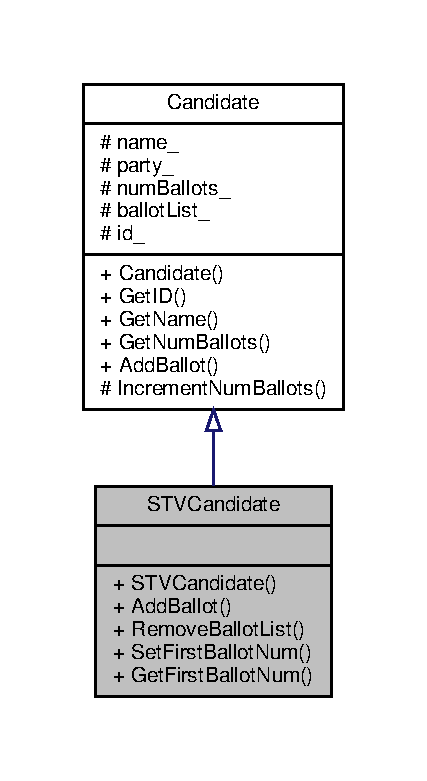
\includegraphics[width=205pt]{classSTVCandidate__inherit__graph}
\end{center}
\end{figure}


Collaboration diagram for S\+T\+V\+Candidate\+:\nopagebreak
\begin{figure}[H]
\begin{center}
\leavevmode
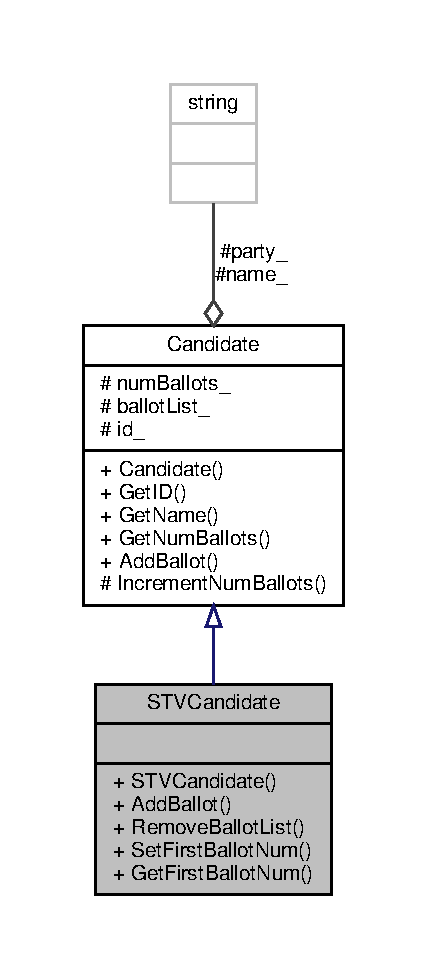
\includegraphics[width=205pt]{classSTVCandidate__coll__graph}
\end{center}
\end{figure}
\subsection*{Public Member Functions}
\begin{DoxyCompactItemize}
\item 
\hyperlink{classSTVCandidate_af9d9b827835e1689069c6fe97a950321}{S\+T\+V\+Candidate} (int, std\+::string, std\+::string)
\begin{DoxyCompactList}\small\item\em Constructs an S\+TV candidate to be used in an S\+TV election. \end{DoxyCompactList}\item 
int \hyperlink{classSTVCandidate_a91601ba711e655bde45114cf846e2787}{Add\+Ballot} (\hyperlink{classBallot}{Ballot} $\ast$ballot)
\begin{DoxyCompactList}\small\item\em Add a ballot to the list of ballots the candidate has. \end{DoxyCompactList}\item 
std\+::list$<$ \hyperlink{classBallot}{Ballot} $\ast$ $>$ \hyperlink{classSTVCandidate_a4eac28947d47e9726a4c0565c7e60250}{Remove\+Ballot\+List} ()
\begin{DoxyCompactList}\small\item\em Remove the list of ballots an S\+TV candidate has. \end{DoxyCompactList}\item 
void \hyperlink{classSTVCandidate_af57688ad8fabeeff8c6738779c7bdc3e}{Set\+First\+Ballot\+Num} (int)
\begin{DoxyCompactList}\small\item\em Save ballot id number for the first ballot given to an S\+TV candiate. \end{DoxyCompactList}\item 
int \hyperlink{classSTVCandidate_a3281dae3d03733994405241e57a23eec}{Get\+First\+Ballot\+Num} () const
\begin{DoxyCompactList}\small\item\em Get the ballot id of the first ballot given to the S\+TV candidate. \end{DoxyCompactList}\end{DoxyCompactItemize}
\subsection*{Additional Inherited Members}


\subsection{Detailed Description}
The main class for S\+TV candidates. 

Is an S\+TV candidate. 

\subsection{Constructor \& Destructor Documentation}
\mbox{\Hypertarget{classSTVCandidate_af9d9b827835e1689069c6fe97a950321}\label{classSTVCandidate_af9d9b827835e1689069c6fe97a950321}} 
\index{S\+T\+V\+Candidate@{S\+T\+V\+Candidate}!S\+T\+V\+Candidate@{S\+T\+V\+Candidate}}
\index{S\+T\+V\+Candidate@{S\+T\+V\+Candidate}!S\+T\+V\+Candidate@{S\+T\+V\+Candidate}}
\subsubsection{\texorpdfstring{S\+T\+V\+Candidate()}{STVCandidate()}}
{\footnotesize\ttfamily S\+T\+V\+Candidate\+::\+S\+T\+V\+Candidate (\begin{DoxyParamCaption}\item[{int}]{candidate\+\_\+num,  }\item[{std\+::string}]{candidate\+\_\+name,  }\item[{std\+::string}]{candidate\+\_\+party }\end{DoxyParamCaption})\hspace{0.3cm}{\ttfamily [explicit]}}



Constructs an S\+TV candidate to be used in an S\+TV election. 


\begin{DoxyParams}[1]{Parameters}
\mbox{\tt in}  & {\em int} & holding an S\+TV candidate id number \\
\hline
\mbox{\tt in}  & {\em string} & containing the S\+TV candidate\textquotesingle{}s name \\
\hline
\mbox{\tt in}  & {\em string} & containing the S\+TV candidate\textquotesingle{}s party \\
\hline
\end{DoxyParams}


\subsection{Member Function Documentation}
\mbox{\Hypertarget{classSTVCandidate_a91601ba711e655bde45114cf846e2787}\label{classSTVCandidate_a91601ba711e655bde45114cf846e2787}} 
\index{S\+T\+V\+Candidate@{S\+T\+V\+Candidate}!Add\+Ballot@{Add\+Ballot}}
\index{Add\+Ballot@{Add\+Ballot}!S\+T\+V\+Candidate@{S\+T\+V\+Candidate}}
\subsubsection{\texorpdfstring{Add\+Ballot()}{AddBallot()}}
{\footnotesize\ttfamily int S\+T\+V\+Candidate\+::\+Add\+Ballot (\begin{DoxyParamCaption}\item[{\hyperlink{classBallot}{Ballot} $\ast$}]{ballot }\end{DoxyParamCaption})}



Add a ballot to the list of ballots the candidate has. 


\begin{DoxyParams}[1]{Parameters}
\mbox{\tt in}  & {\em A} & ballot object \\
\hline
\end{DoxyParams}
\begin{DoxyReturn}{Returns}
int of the number of ballots the candidate has 
\end{DoxyReturn}
\mbox{\Hypertarget{classSTVCandidate_a3281dae3d03733994405241e57a23eec}\label{classSTVCandidate_a3281dae3d03733994405241e57a23eec}} 
\index{S\+T\+V\+Candidate@{S\+T\+V\+Candidate}!Get\+First\+Ballot\+Num@{Get\+First\+Ballot\+Num}}
\index{Get\+First\+Ballot\+Num@{Get\+First\+Ballot\+Num}!S\+T\+V\+Candidate@{S\+T\+V\+Candidate}}
\subsubsection{\texorpdfstring{Get\+First\+Ballot\+Num()}{GetFirstBallotNum()}}
{\footnotesize\ttfamily int S\+T\+V\+Candidate\+::\+Get\+First\+Ballot\+Num (\begin{DoxyParamCaption}{ }\end{DoxyParamCaption}) const}



Get the ballot id of the first ballot given to the S\+TV candidate. 

\begin{DoxyReturn}{Returns}
int of the ballot id number. 
\end{DoxyReturn}
\mbox{\Hypertarget{classSTVCandidate_a4eac28947d47e9726a4c0565c7e60250}\label{classSTVCandidate_a4eac28947d47e9726a4c0565c7e60250}} 
\index{S\+T\+V\+Candidate@{S\+T\+V\+Candidate}!Remove\+Ballot\+List@{Remove\+Ballot\+List}}
\index{Remove\+Ballot\+List@{Remove\+Ballot\+List}!S\+T\+V\+Candidate@{S\+T\+V\+Candidate}}
\subsubsection{\texorpdfstring{Remove\+Ballot\+List()}{RemoveBallotList()}}
{\footnotesize\ttfamily std\+::list$<$ \hyperlink{classBallot}{Ballot} $\ast$ $>$ S\+T\+V\+Candidate\+::\+Remove\+Ballot\+List (\begin{DoxyParamCaption}{ }\end{DoxyParamCaption})}



Remove the list of ballots an S\+TV candidate has. 

\begin{DoxyReturn}{Returns}
list of ballots 
\end{DoxyReturn}
\mbox{\Hypertarget{classSTVCandidate_af57688ad8fabeeff8c6738779c7bdc3e}\label{classSTVCandidate_af57688ad8fabeeff8c6738779c7bdc3e}} 
\index{S\+T\+V\+Candidate@{S\+T\+V\+Candidate}!Set\+First\+Ballot\+Num@{Set\+First\+Ballot\+Num}}
\index{Set\+First\+Ballot\+Num@{Set\+First\+Ballot\+Num}!S\+T\+V\+Candidate@{S\+T\+V\+Candidate}}
\subsubsection{\texorpdfstring{Set\+First\+Ballot\+Num()}{SetFirstBallotNum()}}
{\footnotesize\ttfamily void S\+T\+V\+Candidate\+::\+Set\+First\+Ballot\+Num (\begin{DoxyParamCaption}\item[{int}]{ballot\+\_\+num }\end{DoxyParamCaption})}



Save ballot id number for the first ballot given to an S\+TV candiate. 


\begin{DoxyParams}[1]{Parameters}
\mbox{\tt in}  & {\em the} & ballot id number as an integer. \\
\hline
\end{DoxyParams}


The documentation for this class was generated from the following files\+:\begin{DoxyCompactItemize}
\item 
/home/spitz123/csci5801\+\_\+s20/repo-\/\+Team3/\+Project2/src/\hyperlink{candidate_8h}{candidate.\+h}\item 
/home/spitz123/csci5801\+\_\+s20/repo-\/\+Team3/\+Project2/src/\hyperlink{candidate_8cc}{candidate.\+cc}\end{DoxyCompactItemize}

\hypertarget{classSTVElection}{}\section{S\+T\+V\+Election Class Reference}
\label{classSTVElection}\index{S\+T\+V\+Election@{S\+T\+V\+Election}}


The main class for stv election.  




{\ttfamily \#include $<$stv\+\_\+election.\+h$>$}



Collaboration diagram for S\+T\+V\+Election\+:\nopagebreak
\begin{figure}[H]
\begin{center}
\leavevmode
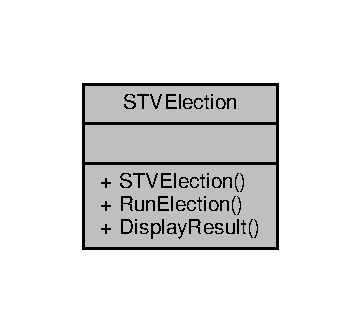
\includegraphics[width=173pt]{classSTVElection__coll__graph}
\end{center}
\end{figure}
\subsection*{Public Member Functions}
\begin{DoxyCompactItemize}
\item 
\hyperlink{classSTVElection_a6abe30e81059242a53f0c06c29331d10}{S\+T\+V\+Election} (\hyperlink{classVotingInfo}{Voting\+Info} $\ast$)
\begin{DoxyCompactList}\small\item\em Constructs an stvelection object to be used in an election. \end{DoxyCompactList}\item 
void \hyperlink{classSTVElection_a3b80c78d70ba3dc7181884b0dfcf142e}{Run\+Election} ()
\begin{DoxyCompactList}\small\item\em Run an S\+TV election. \end{DoxyCompactList}\item 
void \hyperlink{classSTVElection_a224ba2c99b4dbd2f4bbce4de8b1e98f4}{Display\+Result} ()
\begin{DoxyCompactList}\small\item\em Display S\+TV election results. \end{DoxyCompactList}\end{DoxyCompactItemize}


\subsection{Detailed Description}
The main class for stv election. 

Is an stvelection. 

\subsection{Constructor \& Destructor Documentation}
\mbox{\Hypertarget{classSTVElection_a6abe30e81059242a53f0c06c29331d10}\label{classSTVElection_a6abe30e81059242a53f0c06c29331d10}} 
\index{S\+T\+V\+Election@{S\+T\+V\+Election}!S\+T\+V\+Election@{S\+T\+V\+Election}}
\index{S\+T\+V\+Election@{S\+T\+V\+Election}!S\+T\+V\+Election@{S\+T\+V\+Election}}
\subsubsection{\texorpdfstring{S\+T\+V\+Election()}{STVElection()}}
{\footnotesize\ttfamily S\+T\+V\+Election\+::\+S\+T\+V\+Election (\begin{DoxyParamCaption}\item[{\hyperlink{classVotingInfo}{Voting\+Info} $\ast$}]{voting\+Info }\end{DoxyParamCaption})\hspace{0.3cm}{\ttfamily [explicit]}}



Constructs an stvelection object to be used in an election. 


\begin{DoxyParams}[1]{Parameters}
\mbox{\tt in}  & {\em Voting\+Info$\ast$} & data structure \\
\hline
\end{DoxyParams}


\subsection{Member Function Documentation}
\mbox{\Hypertarget{classSTVElection_a224ba2c99b4dbd2f4bbce4de8b1e98f4}\label{classSTVElection_a224ba2c99b4dbd2f4bbce4de8b1e98f4}} 
\index{S\+T\+V\+Election@{S\+T\+V\+Election}!Display\+Result@{Display\+Result}}
\index{Display\+Result@{Display\+Result}!S\+T\+V\+Election@{S\+T\+V\+Election}}
\subsubsection{\texorpdfstring{Display\+Result()}{DisplayResult()}}
{\footnotesize\ttfamily void S\+T\+V\+Election\+::\+Display\+Result (\begin{DoxyParamCaption}{ }\end{DoxyParamCaption})}



Display S\+TV election results. 


\begin{DoxyParams}[1]{Parameters}
\mbox{\tt in}  & {\em none,using} & member structure within the same class \\
\hline
\end{DoxyParams}
\begin{DoxyReturn}{Returns}
void 
\end{DoxyReturn}
\mbox{\Hypertarget{classSTVElection_a3b80c78d70ba3dc7181884b0dfcf142e}\label{classSTVElection_a3b80c78d70ba3dc7181884b0dfcf142e}} 
\index{S\+T\+V\+Election@{S\+T\+V\+Election}!Run\+Election@{Run\+Election}}
\index{Run\+Election@{Run\+Election}!S\+T\+V\+Election@{S\+T\+V\+Election}}
\subsubsection{\texorpdfstring{Run\+Election()}{RunElection()}}
{\footnotesize\ttfamily void S\+T\+V\+Election\+::\+Run\+Election (\begin{DoxyParamCaption}{ }\end{DoxyParamCaption})}



Run an S\+TV election. 


\begin{DoxyParams}[1]{Parameters}
\mbox{\tt in}  & {\em none} & \\
\hline
\end{DoxyParams}
\begin{DoxyReturn}{Returns}
void 
\end{DoxyReturn}


The documentation for this class was generated from the following files\+:\begin{DoxyCompactItemize}
\item 
/home/spitz123/csci5801\+\_\+s20/repo-\/\+Team3/\+Project1/src/\hyperlink{stv__election_8h}{stv\+\_\+election.\+h}\item 
/home/spitz123/csci5801\+\_\+s20/repo-\/\+Team3/\+Project1/src/\hyperlink{stv__election_8cc}{stv\+\_\+election.\+cc}\end{DoxyCompactItemize}

\hypertarget{classSTVElectionRecord}{}\section{S\+T\+V\+Election\+Record Class Reference}
\label{classSTVElectionRecord}\index{S\+T\+V\+Election\+Record@{S\+T\+V\+Election\+Record}}


The class for the S\+TV election records.  




{\ttfamily \#include $<$stv\+\_\+election\+\_\+record.\+h$>$}



Collaboration diagram for S\+T\+V\+Election\+Record\+:\nopagebreak
\begin{figure}[H]
\begin{center}
\leavevmode
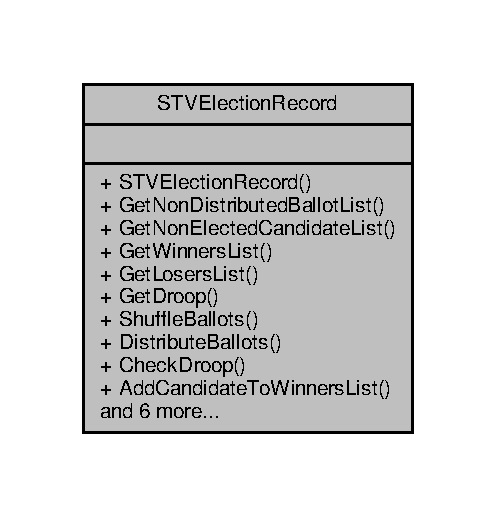
\includegraphics[width=238pt]{classSTVElectionRecord__coll__graph}
\end{center}
\end{figure}
\subsection*{Public Member Functions}
\begin{DoxyCompactItemize}
\item 
\hyperlink{classSTVElectionRecord_a0ede176edc0967c98a23be4754c27e9e}{S\+T\+V\+Election\+Record} (const std\+::list$<$ \hyperlink{classSTVCandidate}{S\+T\+V\+Candidate} $\ast$$>$, const std\+::list$<$ \hyperlink{classBallot}{Ballot} $\ast$$>$, int)
\begin{DoxyCompactList}\small\item\em Constructs an stv election record with a candidate list, ballot list, and droop value. \end{DoxyCompactList}\item 
\mbox{\Hypertarget{classSTVElectionRecord_aacdd25995d5693c501bf1575bf5d1233}\label{classSTVElectionRecord_aacdd25995d5693c501bf1575bf5d1233}} 
std\+::list$<$ \hyperlink{classBallot}{Ballot} $\ast$ $>$ \hyperlink{classSTVElectionRecord_aacdd25995d5693c501bf1575bf5d1233}{Get\+Non\+Distributed\+Ballot\+List} ()
\begin{DoxyCompactList}\small\item\em Function to get non\+Distributed\+Ballot\+List\+\_\+. \end{DoxyCompactList}\item 
\mbox{\Hypertarget{classSTVElectionRecord_ac3c03c1d3a343afbebd43acc1a64fbee}\label{classSTVElectionRecord_ac3c03c1d3a343afbebd43acc1a64fbee}} 
std\+::list$<$ \hyperlink{classSTVCandidate}{S\+T\+V\+Candidate} $\ast$ $>$ \hyperlink{classSTVElectionRecord_ac3c03c1d3a343afbebd43acc1a64fbee}{Get\+Non\+Elected\+Candidate\+List} ()
\begin{DoxyCompactList}\small\item\em Function to get non\+Elected\+Candidate\+List\+\_\+. \end{DoxyCompactList}\item 
\mbox{\Hypertarget{classSTVElectionRecord_a1e1d4ea12462b12789110b1bcd1df580}\label{classSTVElectionRecord_a1e1d4ea12462b12789110b1bcd1df580}} 
std\+::list$<$ \hyperlink{classSTVCandidate}{S\+T\+V\+Candidate} $\ast$ $>$ \hyperlink{classSTVElectionRecord_a1e1d4ea12462b12789110b1bcd1df580}{Get\+Winners\+List} ()
\begin{DoxyCompactList}\small\item\em Function to get winners\+List\+\_\+. \end{DoxyCompactList}\item 
\mbox{\Hypertarget{classSTVElectionRecord_affc79a53b8fa74a8d7a65ae92b256387}\label{classSTVElectionRecord_affc79a53b8fa74a8d7a65ae92b256387}} 
std\+::list$<$ \hyperlink{classSTVCandidate}{S\+T\+V\+Candidate} $\ast$ $>$ \hyperlink{classSTVElectionRecord_affc79a53b8fa74a8d7a65ae92b256387}{Get\+Losers\+List} ()
\begin{DoxyCompactList}\small\item\em Function to get losers\+List\+\_\+. \end{DoxyCompactList}\item 
int \hyperlink{classSTVElectionRecord_aa954f6081a250962261e63a7497c1eb4}{Get\+Droop} ()
\begin{DoxyCompactList}\small\item\em Returns droop quota. \end{DoxyCompactList}\item 
\mbox{\Hypertarget{classSTVElectionRecord_a9f0c214158ad1d590db5f0ac3712c4ef}\label{classSTVElectionRecord_a9f0c214158ad1d590db5f0ac3712c4ef}} 
void \hyperlink{classSTVElectionRecord_a9f0c214158ad1d590db5f0ac3712c4ef}{Shuffle\+Ballots} ()
\begin{DoxyCompactList}\small\item\em Function to shuffle the ballots prior to the election. \end{DoxyCompactList}\item 
\mbox{\Hypertarget{classSTVElectionRecord_a0fb9749e08613f0024656a3b55b9ec3f}\label{classSTVElectionRecord_a0fb9749e08613f0024656a3b55b9ec3f}} 
void \hyperlink{classSTVElectionRecord_a0fb9749e08613f0024656a3b55b9ec3f}{Distribute\+Ballots} (int $\ast$)
\begin{DoxyCompactList}\small\item\em Function to distribute the ballots to the canidate of the ballots choosing. \end{DoxyCompactList}\item 
bool \hyperlink{classSTVElectionRecord_ab941d3821a34ef527128042500c416c7}{Check\+Droop} (int)
\begin{DoxyCompactList}\small\item\em Function to check a ballot count against the droop value. \end{DoxyCompactList}\item 
void \hyperlink{classSTVElectionRecord_af466fd6edc790d7744fe809e7ee9d40c}{Add\+Candidate\+To\+Winners\+List} (\hyperlink{classSTVCandidate}{S\+T\+V\+Candidate} $\ast$)
\begin{DoxyCompactList}\small\item\em Add an stv candidate to the winners list. \end{DoxyCompactList}\item 
\mbox{\Hypertarget{classSTVElectionRecord_a856aa1d361b69b646072579f098b0b3c}\label{classSTVElectionRecord_a856aa1d361b69b646072579f098b0b3c}} 
void \hyperlink{classSTVElectionRecord_a856aa1d361b69b646072579f098b0b3c}{Sort\+Non\+Elected\+Candidate\+List} ()
\begin{DoxyCompactList}\small\item\em Sort the non elected candidate list. \end{DoxyCompactList}\item 
\hyperlink{classSTVCandidate}{S\+T\+V\+Candidate} $\ast$ \hyperlink{classSTVElectionRecord_a741e5d955734ed07db8465cbaa3b0091}{Remove\+Last\+Candidate\+From\+Non\+Elected\+Candidate\+List} ()
\begin{DoxyCompactList}\small\item\em Remove the last candidate from the non elected candidate list. \end{DoxyCompactList}\item 
std\+::list$<$ \hyperlink{classBallot}{Ballot} $\ast$ $>$ \hyperlink{classSTVElectionRecord_a5909386b596e6563a2ec332921133ab6}{Add\+Candidate\+To\+Losers\+List} (\hyperlink{classSTVCandidate}{S\+T\+V\+Candidate} $\ast$)
\begin{DoxyCompactList}\small\item\em Add an stv candidate to the losers list. \end{DoxyCompactList}\item 
void \hyperlink{classSTVElectionRecord_a04c1523f0e9f60e87544542fc39c56c4}{Add\+Loser\+Ballots\+To\+Non\+Distributed\+Ballot\+List} (std\+::list$<$ \hyperlink{classBallot}{Ballot} $\ast$$>$)
\begin{DoxyCompactList}\small\item\em Add the ballots from a losing candidate back into the non distributed ballots list. \end{DoxyCompactList}\item 
void \hyperlink{classSTVElectionRecord_a441b1386f1c250a6e2c92763b31bd1a2}{Add\+Ballot\+To\+Discarded\+Ballot\+List} (\hyperlink{classBallot}{Ballot} $\ast$)
\begin{DoxyCompactList}\small\item\em Add ballot to discared ballot list. \end{DoxyCompactList}\item 
\hyperlink{classSTVCandidate}{S\+T\+V\+Candidate} $\ast$ \hyperlink{classSTVElectionRecord_ae7078fcee0d4b897d1536bee9ac342f6}{Pop\+Candidate\+Off\+Losers\+List} ()
\begin{DoxyCompactList}\small\item\em Take an stv candidate off the losers list. \end{DoxyCompactList}\end{DoxyCompactItemize}


\subsection{Detailed Description}
The class for the S\+TV election records. 

Is an S\+TV Election Record -\/ will do most of S\+TV election work. 

\subsection{Constructor \& Destructor Documentation}
\mbox{\Hypertarget{classSTVElectionRecord_a0ede176edc0967c98a23be4754c27e9e}\label{classSTVElectionRecord_a0ede176edc0967c98a23be4754c27e9e}} 
\index{S\+T\+V\+Election\+Record@{S\+T\+V\+Election\+Record}!S\+T\+V\+Election\+Record@{S\+T\+V\+Election\+Record}}
\index{S\+T\+V\+Election\+Record@{S\+T\+V\+Election\+Record}!S\+T\+V\+Election\+Record@{S\+T\+V\+Election\+Record}}
\subsubsection{\texorpdfstring{S\+T\+V\+Election\+Record()}{STVElectionRecord()}}
{\footnotesize\ttfamily S\+T\+V\+Election\+Record\+::\+S\+T\+V\+Election\+Record (\begin{DoxyParamCaption}\item[{const std\+::list$<$ \hyperlink{classSTVCandidate}{S\+T\+V\+Candidate} $\ast$$>$}]{,  }\item[{const std\+::list$<$ \hyperlink{classBallot}{Ballot} $\ast$$>$}]{,  }\item[{int}]{ }\end{DoxyParamCaption})}



Constructs an stv election record with a candidate list, ballot list, and droop value. 


\begin{DoxyParams}[1]{Parameters}
\mbox{\tt in}  & {\em linked} & list of Candidates \\
\hline
\mbox{\tt in}  & {\em linked} & list of ballots \\
\hline
\mbox{\tt in}  & {\em droop} & value \\
\hline
\end{DoxyParams}


\subsection{Member Function Documentation}
\mbox{\Hypertarget{classSTVElectionRecord_a441b1386f1c250a6e2c92763b31bd1a2}\label{classSTVElectionRecord_a441b1386f1c250a6e2c92763b31bd1a2}} 
\index{S\+T\+V\+Election\+Record@{S\+T\+V\+Election\+Record}!Add\+Ballot\+To\+Discarded\+Ballot\+List@{Add\+Ballot\+To\+Discarded\+Ballot\+List}}
\index{Add\+Ballot\+To\+Discarded\+Ballot\+List@{Add\+Ballot\+To\+Discarded\+Ballot\+List}!S\+T\+V\+Election\+Record@{S\+T\+V\+Election\+Record}}
\subsubsection{\texorpdfstring{Add\+Ballot\+To\+Discarded\+Ballot\+List()}{AddBallotToDiscardedBallotList()}}
{\footnotesize\ttfamily void S\+T\+V\+Election\+Record\+::\+Add\+Ballot\+To\+Discarded\+Ballot\+List (\begin{DoxyParamCaption}\item[{\hyperlink{classBallot}{Ballot} $\ast$}]{ballot }\end{DoxyParamCaption})}



Add ballot to discared ballot list. 


\begin{DoxyParams}[1]{Parameters}
\mbox{\tt in}  & {\em A} & ballot \\
\hline
\end{DoxyParams}
\mbox{\Hypertarget{classSTVElectionRecord_a5909386b596e6563a2ec332921133ab6}\label{classSTVElectionRecord_a5909386b596e6563a2ec332921133ab6}} 
\index{S\+T\+V\+Election\+Record@{S\+T\+V\+Election\+Record}!Add\+Candidate\+To\+Losers\+List@{Add\+Candidate\+To\+Losers\+List}}
\index{Add\+Candidate\+To\+Losers\+List@{Add\+Candidate\+To\+Losers\+List}!S\+T\+V\+Election\+Record@{S\+T\+V\+Election\+Record}}
\subsubsection{\texorpdfstring{Add\+Candidate\+To\+Losers\+List()}{AddCandidateToLosersList()}}
{\footnotesize\ttfamily std\+::list$<$ \hyperlink{classBallot}{Ballot} $\ast$ $>$ S\+T\+V\+Election\+Record\+::\+Add\+Candidate\+To\+Losers\+List (\begin{DoxyParamCaption}\item[{\hyperlink{classSTVCandidate}{S\+T\+V\+Candidate} $\ast$}]{candidate }\end{DoxyParamCaption})}



Add an stv candidate to the losers list. 


\begin{DoxyParams}[1]{Parameters}
\mbox{\tt in}  & {\em an} & stv candidate\\
\hline
\end{DoxyParams}
\begin{DoxyReturn}{Returns}
A list of the losers ballots. 
\end{DoxyReturn}
\mbox{\Hypertarget{classSTVElectionRecord_af466fd6edc790d7744fe809e7ee9d40c}\label{classSTVElectionRecord_af466fd6edc790d7744fe809e7ee9d40c}} 
\index{S\+T\+V\+Election\+Record@{S\+T\+V\+Election\+Record}!Add\+Candidate\+To\+Winners\+List@{Add\+Candidate\+To\+Winners\+List}}
\index{Add\+Candidate\+To\+Winners\+List@{Add\+Candidate\+To\+Winners\+List}!S\+T\+V\+Election\+Record@{S\+T\+V\+Election\+Record}}
\subsubsection{\texorpdfstring{Add\+Candidate\+To\+Winners\+List()}{AddCandidateToWinnersList()}}
{\footnotesize\ttfamily void S\+T\+V\+Election\+Record\+::\+Add\+Candidate\+To\+Winners\+List (\begin{DoxyParamCaption}\item[{\hyperlink{classSTVCandidate}{S\+T\+V\+Candidate} $\ast$}]{candidate }\end{DoxyParamCaption})}



Add an stv candidate to the winners list. 


\begin{DoxyParams}[1]{Parameters}
\mbox{\tt in}  & {\em An} & stv candidate \\
\hline
\end{DoxyParams}
\mbox{\Hypertarget{classSTVElectionRecord_a04c1523f0e9f60e87544542fc39c56c4}\label{classSTVElectionRecord_a04c1523f0e9f60e87544542fc39c56c4}} 
\index{S\+T\+V\+Election\+Record@{S\+T\+V\+Election\+Record}!Add\+Loser\+Ballots\+To\+Non\+Distributed\+Ballot\+List@{Add\+Loser\+Ballots\+To\+Non\+Distributed\+Ballot\+List}}
\index{Add\+Loser\+Ballots\+To\+Non\+Distributed\+Ballot\+List@{Add\+Loser\+Ballots\+To\+Non\+Distributed\+Ballot\+List}!S\+T\+V\+Election\+Record@{S\+T\+V\+Election\+Record}}
\subsubsection{\texorpdfstring{Add\+Loser\+Ballots\+To\+Non\+Distributed\+Ballot\+List()}{AddLoserBallotsToNonDistributedBallotList()}}
{\footnotesize\ttfamily void S\+T\+V\+Election\+Record\+::\+Add\+Loser\+Ballots\+To\+Non\+Distributed\+Ballot\+List (\begin{DoxyParamCaption}\item[{std\+::list$<$ \hyperlink{classBallot}{Ballot} $\ast$$>$}]{ballot\+\_\+list }\end{DoxyParamCaption})}



Add the ballots from a losing candidate back into the non distributed ballots list. 


\begin{DoxyParams}[1]{Parameters}
\mbox{\tt in}  & {\em A} & list of ballots \\
\hline
\end{DoxyParams}
\mbox{\Hypertarget{classSTVElectionRecord_ab941d3821a34ef527128042500c416c7}\label{classSTVElectionRecord_ab941d3821a34ef527128042500c416c7}} 
\index{S\+T\+V\+Election\+Record@{S\+T\+V\+Election\+Record}!Check\+Droop@{Check\+Droop}}
\index{Check\+Droop@{Check\+Droop}!S\+T\+V\+Election\+Record@{S\+T\+V\+Election\+Record}}
\subsubsection{\texorpdfstring{Check\+Droop()}{CheckDroop()}}
{\footnotesize\ttfamily bool S\+T\+V\+Election\+Record\+::\+Check\+Droop (\begin{DoxyParamCaption}\item[{int}]{droop }\end{DoxyParamCaption})}



Function to check a ballot count against the droop value. 


\begin{DoxyParams}[1]{Parameters}
\mbox{\tt in}  & {\em A} & ballot count.\\
\hline
\end{DoxyParams}
\begin{DoxyReturn}{Returns}
Returns a bool of true if droop has been met and false otherwise. 
\end{DoxyReturn}
\mbox{\Hypertarget{classSTVElectionRecord_aa954f6081a250962261e63a7497c1eb4}\label{classSTVElectionRecord_aa954f6081a250962261e63a7497c1eb4}} 
\index{S\+T\+V\+Election\+Record@{S\+T\+V\+Election\+Record}!Get\+Droop@{Get\+Droop}}
\index{Get\+Droop@{Get\+Droop}!S\+T\+V\+Election\+Record@{S\+T\+V\+Election\+Record}}
\subsubsection{\texorpdfstring{Get\+Droop()}{GetDroop()}}
{\footnotesize\ttfamily int S\+T\+V\+Election\+Record\+::\+Get\+Droop (\begin{DoxyParamCaption}{ }\end{DoxyParamCaption})}



Returns droop quota. 

\begin{DoxyReturn}{Returns}
int holding droop quota. 
\end{DoxyReturn}
\mbox{\Hypertarget{classSTVElectionRecord_ae7078fcee0d4b897d1536bee9ac342f6}\label{classSTVElectionRecord_ae7078fcee0d4b897d1536bee9ac342f6}} 
\index{S\+T\+V\+Election\+Record@{S\+T\+V\+Election\+Record}!Pop\+Candidate\+Off\+Losers\+List@{Pop\+Candidate\+Off\+Losers\+List}}
\index{Pop\+Candidate\+Off\+Losers\+List@{Pop\+Candidate\+Off\+Losers\+List}!S\+T\+V\+Election\+Record@{S\+T\+V\+Election\+Record}}
\subsubsection{\texorpdfstring{Pop\+Candidate\+Off\+Losers\+List()}{PopCandidateOffLosersList()}}
{\footnotesize\ttfamily \hyperlink{classSTVCandidate}{S\+T\+V\+Candidate} $\ast$ S\+T\+V\+Election\+Record\+::\+Pop\+Candidate\+Off\+Losers\+List (\begin{DoxyParamCaption}{ }\end{DoxyParamCaption})}



Take an stv candidate off the losers list. 

\begin{DoxyReturn}{Returns}
An stv candidate 
\end{DoxyReturn}
\mbox{\Hypertarget{classSTVElectionRecord_a741e5d955734ed07db8465cbaa3b0091}\label{classSTVElectionRecord_a741e5d955734ed07db8465cbaa3b0091}} 
\index{S\+T\+V\+Election\+Record@{S\+T\+V\+Election\+Record}!Remove\+Last\+Candidate\+From\+Non\+Elected\+Candidate\+List@{Remove\+Last\+Candidate\+From\+Non\+Elected\+Candidate\+List}}
\index{Remove\+Last\+Candidate\+From\+Non\+Elected\+Candidate\+List@{Remove\+Last\+Candidate\+From\+Non\+Elected\+Candidate\+List}!S\+T\+V\+Election\+Record@{S\+T\+V\+Election\+Record}}
\subsubsection{\texorpdfstring{Remove\+Last\+Candidate\+From\+Non\+Elected\+Candidate\+List()}{RemoveLastCandidateFromNonElectedCandidateList()}}
{\footnotesize\ttfamily \hyperlink{classSTVCandidate}{S\+T\+V\+Candidate} $\ast$ S\+T\+V\+Election\+Record\+::\+Remove\+Last\+Candidate\+From\+Non\+Elected\+Candidate\+List (\begin{DoxyParamCaption}{ }\end{DoxyParamCaption})}



Remove the last candidate from the non elected candidate list. 

\begin{DoxyReturn}{Returns}
The last stv candidate from the non elected candidates list 
\end{DoxyReturn}


The documentation for this class was generated from the following files\+:\begin{DoxyCompactItemize}
\item 
/home/spitz123/csci5801\+\_\+s20/repo-\/\+Team3/\+Project2/src/\hyperlink{stv__election__record_8h}{stv\+\_\+election\+\_\+record.\+h}\item 
/home/spitz123/csci5801\+\_\+s20/repo-\/\+Team3/\+Project2/src/stv\+\_\+election\+\_\+record.\+cc\end{DoxyCompactItemize}

\hypertarget{classVotingInfo}{}\section{Voting\+Info Class Reference}
\label{classVotingInfo}\index{Voting\+Info@{Voting\+Info}}


The main class for storing voting information.  




{\ttfamily \#include $<$voting\+\_\+info.\+h$>$}



Collaboration diagram for Voting\+Info\+:\nopagebreak
\begin{figure}[H]
\begin{center}
\leavevmode
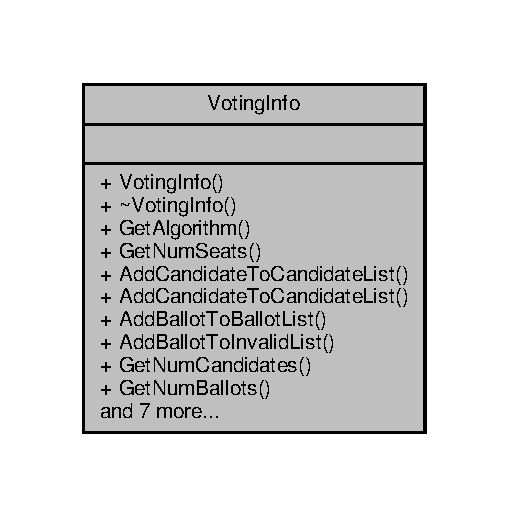
\includegraphics[width=244pt]{classVotingInfo__coll__graph}
\end{center}
\end{figure}
\subsection*{Public Member Functions}
\begin{DoxyCompactItemize}
\item 
\hyperlink{classVotingInfo_a7bdb2f2026f5f68eee3fbee92855b759}{Voting\+Info} (int=-\/1, int=-\/1)
\begin{DoxyCompactList}\small\item\em Constructs a voting info container with an algorithm choice and number of seats available. \end{DoxyCompactList}\item 
\mbox{\Hypertarget{classVotingInfo_a72e88f41ab4e266582041b8f42768586}\label{classVotingInfo_a72e88f41ab4e266582041b8f42768586}} 
\hyperlink{classVotingInfo_a72e88f41ab4e266582041b8f42768586}{$\sim$\+Voting\+Info} ()
\begin{DoxyCompactList}\small\item\em Deconstructs a voting info container. \end{DoxyCompactList}\item 
int \hyperlink{classVotingInfo_a2d0abd1d9be36bfd9fb734dfa644b8e1}{Get\+Algorithm} () const
\begin{DoxyCompactList}\small\item\em Returns choice of algorithm. \end{DoxyCompactList}\item 
int \hyperlink{classVotingInfo_a9c226e3b169e0228ab26cb0a251792bd}{Get\+Num\+Seats} () const
\begin{DoxyCompactList}\small\item\em Returns number of seats available. \end{DoxyCompactList}\item 
void \hyperlink{classVotingInfo_ac0ab5f83a06ea6721999addb43a581ea}{Add\+Candidate\+To\+Candidate\+List} (\hyperlink{classCandidate}{Candidate} $\ast$)
\begin{DoxyCompactList}\small\item\em Adds a candidate to the list of candidates. \end{DoxyCompactList}\item 
void \hyperlink{classVotingInfo_a18d8dfef16797ef988a296d5ef28c852}{Add\+Candidate\+To\+Candidate\+List} (\hyperlink{classSTVCandidate}{S\+T\+V\+Candidate} $\ast$)
\begin{DoxyCompactList}\small\item\em Adds an S\+TV candidate to the list of candidates. \end{DoxyCompactList}\item 
void \hyperlink{classVotingInfo_ae4b8b9a77642271760bce59a0411f900}{Add\+Ballot\+To\+Ballot\+List} (\hyperlink{classBallot}{Ballot} $\ast$)
\begin{DoxyCompactList}\small\item\em Adds a ballot to the list of ballots. \end{DoxyCompactList}\item 
int \hyperlink{classVotingInfo_add7749e53650135da703aa7b816598f5}{Get\+Num\+Candidates} () const
\begin{DoxyCompactList}\small\item\em Returns number of candidates in candidate list. \end{DoxyCompactList}\item 
int \hyperlink{classVotingInfo_af84ccfdfbdf95bc33f959d8b82e27d8c}{Get\+Num\+Ballots} () const
\begin{DoxyCompactList}\small\item\em Returns number of ballots in ballot list. \end{DoxyCompactList}\item 
std\+::list$<$ \hyperlink{classCandidate}{Candidate} $\ast$ $>$ \hyperlink{classVotingInfo_ad64e934ebd73e4be9e89458e0a304030}{Get\+Candidate\+List} () const
\begin{DoxyCompactList}\small\item\em Returns list of candidates. \end{DoxyCompactList}\item 
std\+::list$<$ \hyperlink{classSTVCandidate}{S\+T\+V\+Candidate} $\ast$ $>$ \hyperlink{classVotingInfo_a16f743613daad52be36a92226001e5dd}{Get\+S\+T\+V\+Candidate\+List} () const
\begin{DoxyCompactList}\small\item\em Returns list of S\+TV candidates. \end{DoxyCompactList}\item 
std\+::list$<$ \hyperlink{classBallot}{Ballot} $\ast$ $>$ \hyperlink{classVotingInfo_a73ac1888c3695a912ef6991b6667eeaf}{Get\+Ballot\+List} () const
\begin{DoxyCompactList}\small\item\em Returns list of ballots. \end{DoxyCompactList}\end{DoxyCompactItemize}


\subsection{Detailed Description}
The main class for storing voting information. 

Is a voting information container. 

\subsection{Constructor \& Destructor Documentation}
\mbox{\Hypertarget{classVotingInfo_a7bdb2f2026f5f68eee3fbee92855b759}\label{classVotingInfo_a7bdb2f2026f5f68eee3fbee92855b759}} 
\index{Voting\+Info@{Voting\+Info}!Voting\+Info@{Voting\+Info}}
\index{Voting\+Info@{Voting\+Info}!Voting\+Info@{Voting\+Info}}
\subsubsection{\texorpdfstring{Voting\+Info()}{VotingInfo()}}
{\footnotesize\ttfamily Voting\+Info\+::\+Voting\+Info (\begin{DoxyParamCaption}\item[{int}]{algorithm = {\ttfamily -\/1},  }\item[{int}]{seats = {\ttfamily -\/1} }\end{DoxyParamCaption})\hspace{0.3cm}{\ttfamily [explicit]}}



Constructs a voting info container with an algorithm choice and number of seats available. 


\begin{DoxyParams}[1]{Parameters}
\mbox{\tt in}  & {\em int} & holding choice of algorithm (0 for plurality, 1 for S\+TV). \\
\hline
\mbox{\tt in}  & {\em int} & holding number of seats available. \\
\hline
\end{DoxyParams}


\subsection{Member Function Documentation}
\mbox{\Hypertarget{classVotingInfo_ae4b8b9a77642271760bce59a0411f900}\label{classVotingInfo_ae4b8b9a77642271760bce59a0411f900}} 
\index{Voting\+Info@{Voting\+Info}!Add\+Ballot\+To\+Ballot\+List@{Add\+Ballot\+To\+Ballot\+List}}
\index{Add\+Ballot\+To\+Ballot\+List@{Add\+Ballot\+To\+Ballot\+List}!Voting\+Info@{Voting\+Info}}
\subsubsection{\texorpdfstring{Add\+Ballot\+To\+Ballot\+List()}{AddBallotToBallotList()}}
{\footnotesize\ttfamily void Voting\+Info\+::\+Add\+Ballot\+To\+Ballot\+List (\begin{DoxyParamCaption}\item[{\hyperlink{classBallot}{Ballot} $\ast$}]{ballot }\end{DoxyParamCaption})}



Adds a ballot to the list of ballots. 


\begin{DoxyParams}[1]{Parameters}
\mbox{\tt in}  & {\em Ballot$\ast$} & holding a ballot to be added. \\
\hline
\end{DoxyParams}
\mbox{\Hypertarget{classVotingInfo_ac0ab5f83a06ea6721999addb43a581ea}\label{classVotingInfo_ac0ab5f83a06ea6721999addb43a581ea}} 
\index{Voting\+Info@{Voting\+Info}!Add\+Candidate\+To\+Candidate\+List@{Add\+Candidate\+To\+Candidate\+List}}
\index{Add\+Candidate\+To\+Candidate\+List@{Add\+Candidate\+To\+Candidate\+List}!Voting\+Info@{Voting\+Info}}
\subsubsection{\texorpdfstring{Add\+Candidate\+To\+Candidate\+List()}{AddCandidateToCandidateList()}\hspace{0.1cm}{\footnotesize\ttfamily [1/2]}}
{\footnotesize\ttfamily void Voting\+Info\+::\+Add\+Candidate\+To\+Candidate\+List (\begin{DoxyParamCaption}\item[{\hyperlink{classCandidate}{Candidate} $\ast$}]{candidate }\end{DoxyParamCaption})}



Adds a candidate to the list of candidates. 


\begin{DoxyParams}[1]{Parameters}
\mbox{\tt in}  & {\em Candidate$\ast$} & holding a candidate to be added. \\
\hline
\end{DoxyParams}
\mbox{\Hypertarget{classVotingInfo_a18d8dfef16797ef988a296d5ef28c852}\label{classVotingInfo_a18d8dfef16797ef988a296d5ef28c852}} 
\index{Voting\+Info@{Voting\+Info}!Add\+Candidate\+To\+Candidate\+List@{Add\+Candidate\+To\+Candidate\+List}}
\index{Add\+Candidate\+To\+Candidate\+List@{Add\+Candidate\+To\+Candidate\+List}!Voting\+Info@{Voting\+Info}}
\subsubsection{\texorpdfstring{Add\+Candidate\+To\+Candidate\+List()}{AddCandidateToCandidateList()}\hspace{0.1cm}{\footnotesize\ttfamily [2/2]}}
{\footnotesize\ttfamily void Voting\+Info\+::\+Add\+Candidate\+To\+Candidate\+List (\begin{DoxyParamCaption}\item[{\hyperlink{classSTVCandidate}{S\+T\+V\+Candidate} $\ast$}]{stv\+\_\+candidate }\end{DoxyParamCaption})}



Adds an S\+TV candidate to the list of candidates. 


\begin{DoxyParams}[1]{Parameters}
\mbox{\tt in}  & {\em S\+T\+V\+Candidate$\ast$} & holding an S\+TV candidate to be added. \\
\hline
\end{DoxyParams}
\mbox{\Hypertarget{classVotingInfo_a2d0abd1d9be36bfd9fb734dfa644b8e1}\label{classVotingInfo_a2d0abd1d9be36bfd9fb734dfa644b8e1}} 
\index{Voting\+Info@{Voting\+Info}!Get\+Algorithm@{Get\+Algorithm}}
\index{Get\+Algorithm@{Get\+Algorithm}!Voting\+Info@{Voting\+Info}}
\subsubsection{\texorpdfstring{Get\+Algorithm()}{GetAlgorithm()}}
{\footnotesize\ttfamily int Voting\+Info\+::\+Get\+Algorithm (\begin{DoxyParamCaption}{ }\end{DoxyParamCaption}) const}



Returns choice of algorithm. 

\begin{DoxyReturn}{Returns}
int holding choice of algorithm (0 for plurality, 1 for S\+TV). 
\end{DoxyReturn}
\mbox{\Hypertarget{classVotingInfo_a73ac1888c3695a912ef6991b6667eeaf}\label{classVotingInfo_a73ac1888c3695a912ef6991b6667eeaf}} 
\index{Voting\+Info@{Voting\+Info}!Get\+Ballot\+List@{Get\+Ballot\+List}}
\index{Get\+Ballot\+List@{Get\+Ballot\+List}!Voting\+Info@{Voting\+Info}}
\subsubsection{\texorpdfstring{Get\+Ballot\+List()}{GetBallotList()}}
{\footnotesize\ttfamily std\+::list$<$ \hyperlink{classBallot}{Ballot} $\ast$ $>$ Voting\+Info\+::\+Get\+Ballot\+List (\begin{DoxyParamCaption}{ }\end{DoxyParamCaption}) const}



Returns list of ballots. 

\begin{DoxyReturn}{Returns}
std\+::list$<$\+Ballot$\ast$$>$ holding list of ballots. 
\end{DoxyReturn}
\mbox{\Hypertarget{classVotingInfo_ad64e934ebd73e4be9e89458e0a304030}\label{classVotingInfo_ad64e934ebd73e4be9e89458e0a304030}} 
\index{Voting\+Info@{Voting\+Info}!Get\+Candidate\+List@{Get\+Candidate\+List}}
\index{Get\+Candidate\+List@{Get\+Candidate\+List}!Voting\+Info@{Voting\+Info}}
\subsubsection{\texorpdfstring{Get\+Candidate\+List()}{GetCandidateList()}}
{\footnotesize\ttfamily std\+::list$<$ \hyperlink{classCandidate}{Candidate} $\ast$ $>$ Voting\+Info\+::\+Get\+Candidate\+List (\begin{DoxyParamCaption}{ }\end{DoxyParamCaption}) const}



Returns list of candidates. 

\begin{DoxyReturn}{Returns}
std\+::list$<$\+Candidate$\ast$$>$ holding list of candidates. 
\end{DoxyReturn}
\mbox{\Hypertarget{classVotingInfo_af84ccfdfbdf95bc33f959d8b82e27d8c}\label{classVotingInfo_af84ccfdfbdf95bc33f959d8b82e27d8c}} 
\index{Voting\+Info@{Voting\+Info}!Get\+Num\+Ballots@{Get\+Num\+Ballots}}
\index{Get\+Num\+Ballots@{Get\+Num\+Ballots}!Voting\+Info@{Voting\+Info}}
\subsubsection{\texorpdfstring{Get\+Num\+Ballots()}{GetNumBallots()}}
{\footnotesize\ttfamily int Voting\+Info\+::\+Get\+Num\+Ballots (\begin{DoxyParamCaption}{ }\end{DoxyParamCaption}) const}



Returns number of ballots in ballot list. 

\begin{DoxyReturn}{Returns}
int holding number of ballots in ballot list. 
\end{DoxyReturn}
\mbox{\Hypertarget{classVotingInfo_add7749e53650135da703aa7b816598f5}\label{classVotingInfo_add7749e53650135da703aa7b816598f5}} 
\index{Voting\+Info@{Voting\+Info}!Get\+Num\+Candidates@{Get\+Num\+Candidates}}
\index{Get\+Num\+Candidates@{Get\+Num\+Candidates}!Voting\+Info@{Voting\+Info}}
\subsubsection{\texorpdfstring{Get\+Num\+Candidates()}{GetNumCandidates()}}
{\footnotesize\ttfamily int Voting\+Info\+::\+Get\+Num\+Candidates (\begin{DoxyParamCaption}{ }\end{DoxyParamCaption}) const}



Returns number of candidates in candidate list. 

\begin{DoxyReturn}{Returns}
int holding number of candidates in candidate list. 
\end{DoxyReturn}
\mbox{\Hypertarget{classVotingInfo_a9c226e3b169e0228ab26cb0a251792bd}\label{classVotingInfo_a9c226e3b169e0228ab26cb0a251792bd}} 
\index{Voting\+Info@{Voting\+Info}!Get\+Num\+Seats@{Get\+Num\+Seats}}
\index{Get\+Num\+Seats@{Get\+Num\+Seats}!Voting\+Info@{Voting\+Info}}
\subsubsection{\texorpdfstring{Get\+Num\+Seats()}{GetNumSeats()}}
{\footnotesize\ttfamily int Voting\+Info\+::\+Get\+Num\+Seats (\begin{DoxyParamCaption}{ }\end{DoxyParamCaption}) const}



Returns number of seats available. 

\begin{DoxyReturn}{Returns}
int holding number of seats available. 
\end{DoxyReturn}
\mbox{\Hypertarget{classVotingInfo_a16f743613daad52be36a92226001e5dd}\label{classVotingInfo_a16f743613daad52be36a92226001e5dd}} 
\index{Voting\+Info@{Voting\+Info}!Get\+S\+T\+V\+Candidate\+List@{Get\+S\+T\+V\+Candidate\+List}}
\index{Get\+S\+T\+V\+Candidate\+List@{Get\+S\+T\+V\+Candidate\+List}!Voting\+Info@{Voting\+Info}}
\subsubsection{\texorpdfstring{Get\+S\+T\+V\+Candidate\+List()}{GetSTVCandidateList()}}
{\footnotesize\ttfamily std\+::list$<$ \hyperlink{classSTVCandidate}{S\+T\+V\+Candidate} $\ast$ $>$ Voting\+Info\+::\+Get\+S\+T\+V\+Candidate\+List (\begin{DoxyParamCaption}{ }\end{DoxyParamCaption}) const}



Returns list of S\+TV candidates. 

\begin{DoxyReturn}{Returns}
std\+::list$<$\+S\+T\+V\+Candidate$\ast$$>$ holding list of candidates. 
\end{DoxyReturn}


The documentation for this class was generated from the following files\+:\begin{DoxyCompactItemize}
\item 
/home/spitz123/csci5801\+\_\+s20/repo-\/\+Team3/\+Project1/src/\hyperlink{voting__info_8h}{voting\+\_\+info.\+h}\item 
/home/spitz123/csci5801\+\_\+s20/repo-\/\+Team3/\+Project1/src/\hyperlink{voting__info_8cc}{voting\+\_\+info.\+cc}\end{DoxyCompactItemize}

\chapter{File Documentation}
\hypertarget{ballot_8cc}{}\section{/home/spitz123/csci5801\+\_\+s20/repo-\/\+Team3/\+Project1/src/ballot.cc File Reference}
\label{ballot_8cc}\index{/home/spitz123/csci5801\+\_\+s20/repo-\/\+Team3/\+Project1/src/ballot.\+cc@{/home/spitz123/csci5801\+\_\+s20/repo-\/\+Team3/\+Project1/src/ballot.\+cc}}
{\ttfamily \#include \char`\"{}ballot.\+h\char`\"{}}\newline
Include dependency graph for ballot.\+cc\+:
\nopagebreak
\begin{figure}[H]
\begin{center}
\leavevmode
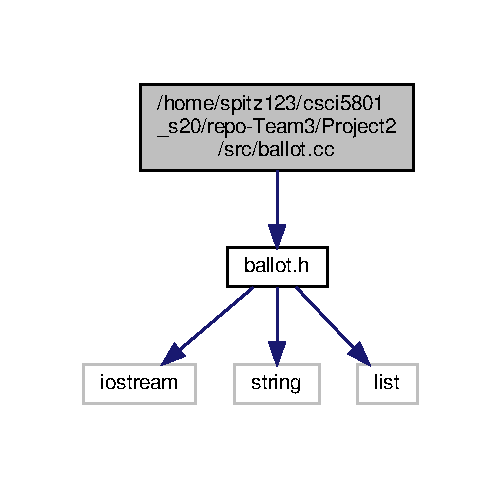
\includegraphics[width=241pt]{ballot_8cc__incl}
\end{center}
\end{figure}


\subsection{Detailed Description}
\begin{DoxyCopyright}{Copyright}
2020 5801 Team3, All rights reserved. 
\end{DoxyCopyright}

\hypertarget{ballot_8h}{}\section{/home/spitz123/csci5801\+\_\+s20/repo-\/\+Team3/\+Project1/src/ballot.h File Reference}
\label{ballot_8h}\index{/home/spitz123/csci5801\+\_\+s20/repo-\/\+Team3/\+Project1/src/ballot.\+h@{/home/spitz123/csci5801\+\_\+s20/repo-\/\+Team3/\+Project1/src/ballot.\+h}}
{\ttfamily \#include $<$iostream$>$}\newline
{\ttfamily \#include $<$string$>$}\newline
{\ttfamily \#include $<$list$>$}\newline
Include dependency graph for ballot.\+h\+:
\nopagebreak
\begin{figure}[H]
\begin{center}
\leavevmode
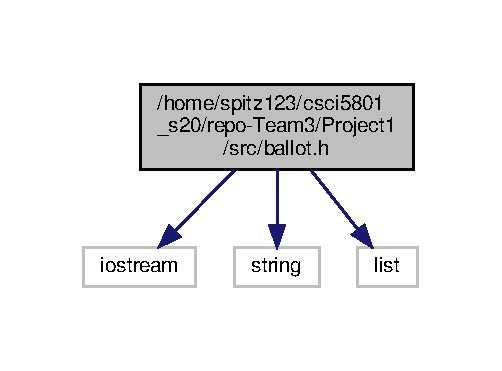
\includegraphics[width=241pt]{ballot_8h__incl}
\end{center}
\end{figure}
This graph shows which files directly or indirectly include this file\+:
\nopagebreak
\begin{figure}[H]
\begin{center}
\leavevmode
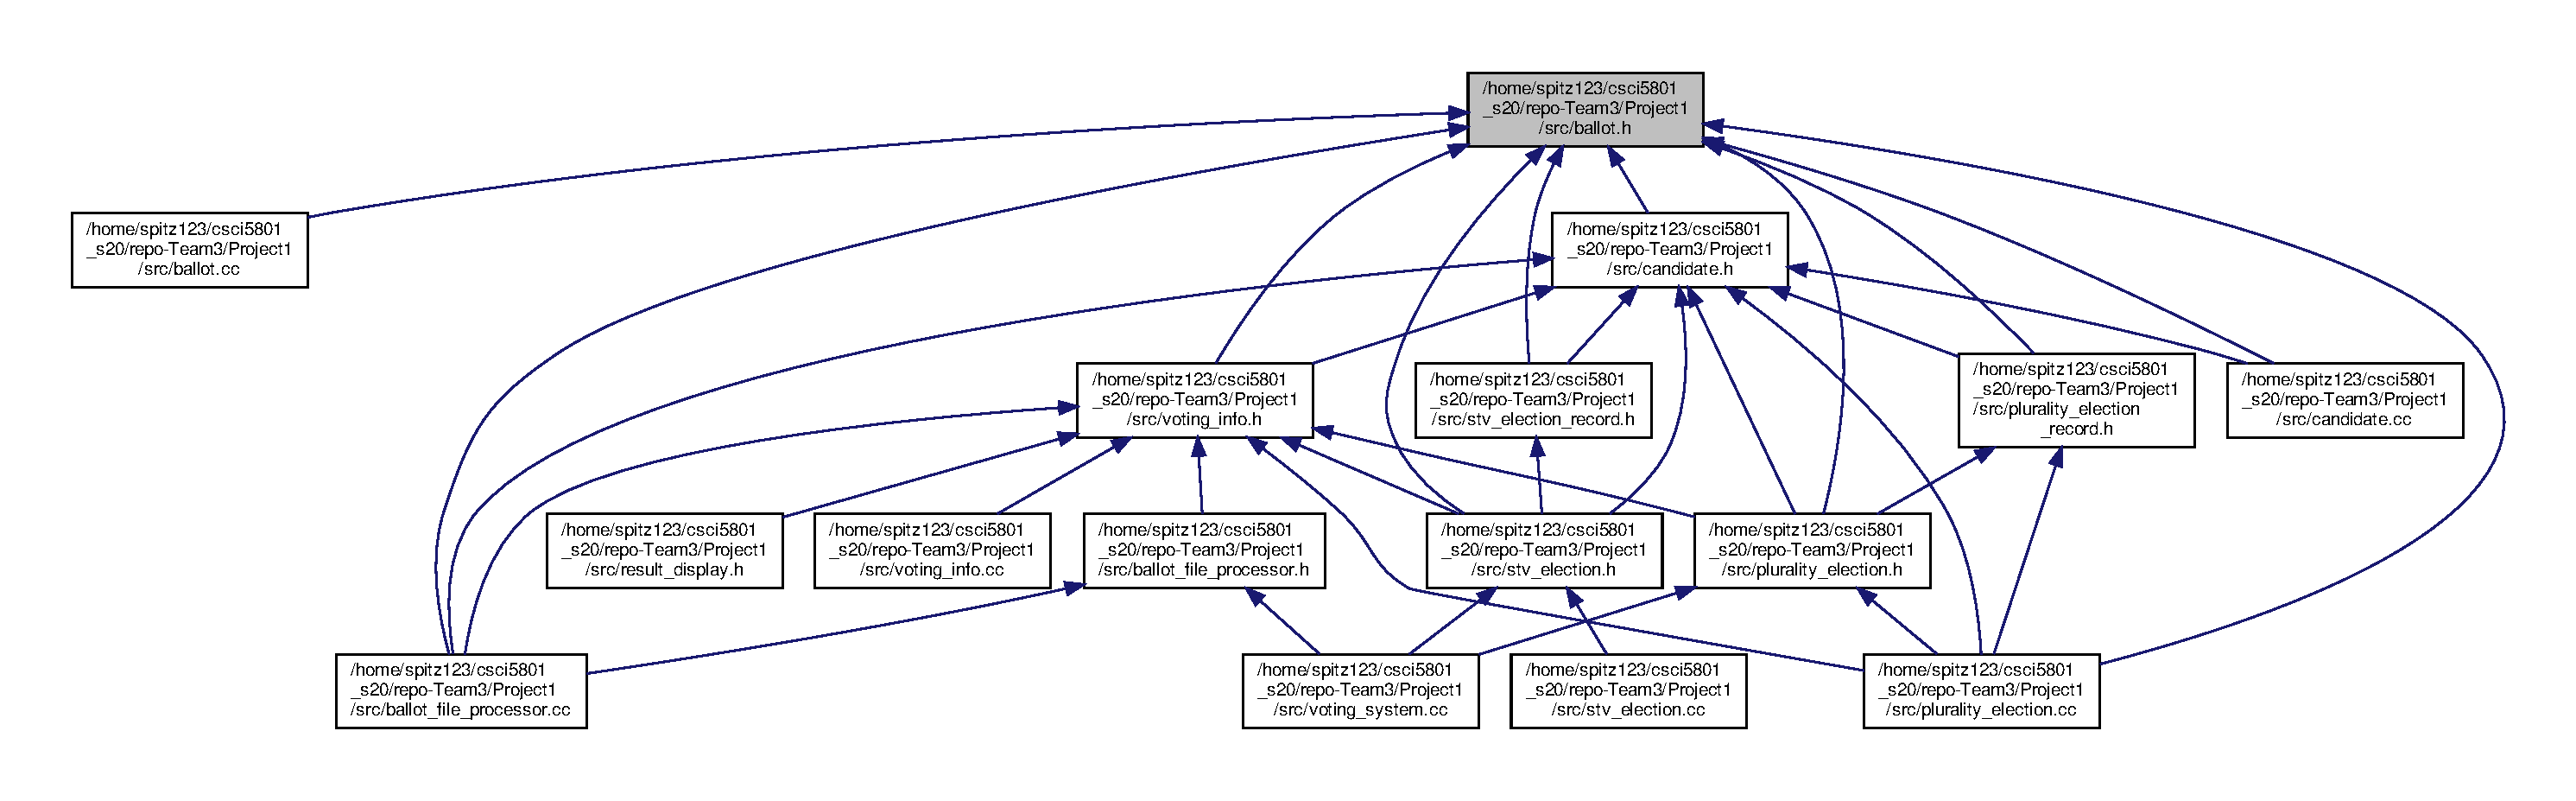
\includegraphics[width=350pt]{ballot_8h__dep__incl}
\end{center}
\end{figure}
\subsection*{Classes}
\begin{DoxyCompactItemize}
\item 
class \hyperlink{classBallot}{Ballot}
\begin{DoxyCompactList}\small\item\em The main class for ballots. \end{DoxyCompactList}\end{DoxyCompactItemize}


\subsection{Detailed Description}
\begin{DoxyCopyright}{Copyright}
2020 5801 Team3, All rights reserved. 
\end{DoxyCopyright}

\hypertarget{ballot__file__processor_8cc}{}\section{/home/spitz123/csci5801\+\_\+s20/repo-\/\+Team3/\+Project2/src/ballot\+\_\+file\+\_\+processor.cc File Reference}
\label{ballot__file__processor_8cc}\index{/home/spitz123/csci5801\+\_\+s20/repo-\/\+Team3/\+Project2/src/ballot\+\_\+file\+\_\+processor.\+cc@{/home/spitz123/csci5801\+\_\+s20/repo-\/\+Team3/\+Project2/src/ballot\+\_\+file\+\_\+processor.\+cc}}
{\ttfamily \#include \char`\"{}ballot\+\_\+file\+\_\+processor.\+h\char`\"{}}\newline
Include dependency graph for ballot\+\_\+file\+\_\+processor.\+cc\+:\nopagebreak
\begin{figure}[H]
\begin{center}
\leavevmode
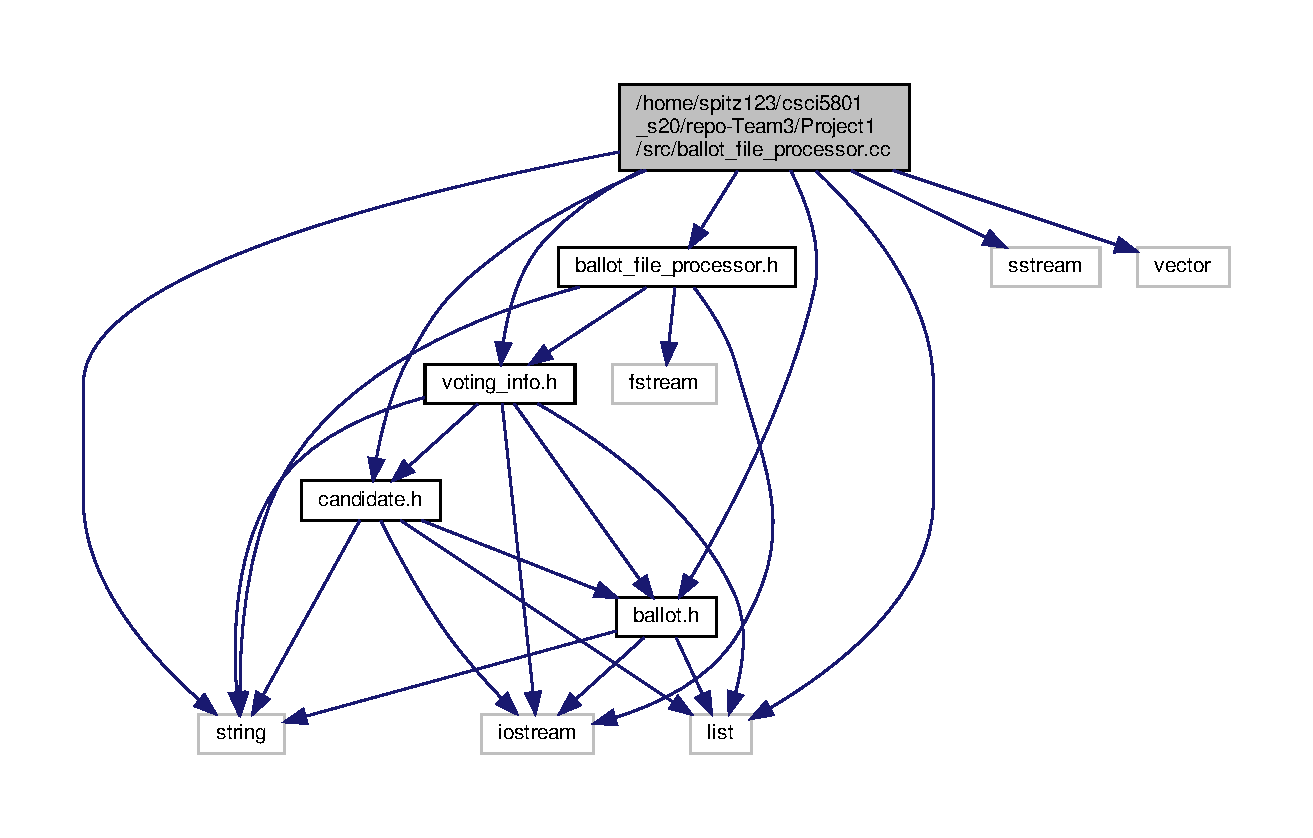
\includegraphics[width=350pt]{ballot__file__processor_8cc__incl}
\end{center}
\end{figure}


\subsection{Detailed Description}
\begin{DoxyCopyright}{Copyright}
2020 5801 Team3, All rights reserved. 
\end{DoxyCopyright}

\hypertarget{ballot__file__processor_8h}{}\section{/home/spitz123/csci5801\+\_\+s20/repo-\/\+Team3/\+Project2/src/ballot\+\_\+file\+\_\+processor.h File Reference}
\label{ballot__file__processor_8h}\index{/home/spitz123/csci5801\+\_\+s20/repo-\/\+Team3/\+Project2/src/ballot\+\_\+file\+\_\+processor.\+h@{/home/spitz123/csci5801\+\_\+s20/repo-\/\+Team3/\+Project2/src/ballot\+\_\+file\+\_\+processor.\+h}}
{\ttfamily \#include $<$fstream$>$}\newline
{\ttfamily \#include $<$string$>$}\newline
{\ttfamily \#include $<$sstream$>$}\newline
{\ttfamily \#include $<$vector$>$}\newline
{\ttfamily \#include $<$list$>$}\newline
{\ttfamily \#include $<$cctype$>$}\newline
{\ttfamily \#include $<$iostream$>$}\newline
{\ttfamily \#include \char`\"{}logger.\+h\char`\"{}}\newline
{\ttfamily \#include $<$dirent.\+h$>$}\newline
{\ttfamily \#include $<$sys/types.\+h$>$}\newline
{\ttfamily \#include \char`\"{}candidate.\+h\char`\"{}}\newline
{\ttfamily \#include \char`\"{}ballot.\+h\char`\"{}}\newline
{\ttfamily \#include \char`\"{}voting\+\_\+info.\+h\char`\"{}}\newline
Include dependency graph for ballot\+\_\+file\+\_\+processor.\+h\+:\nopagebreak
\begin{figure}[H]
\begin{center}
\leavevmode
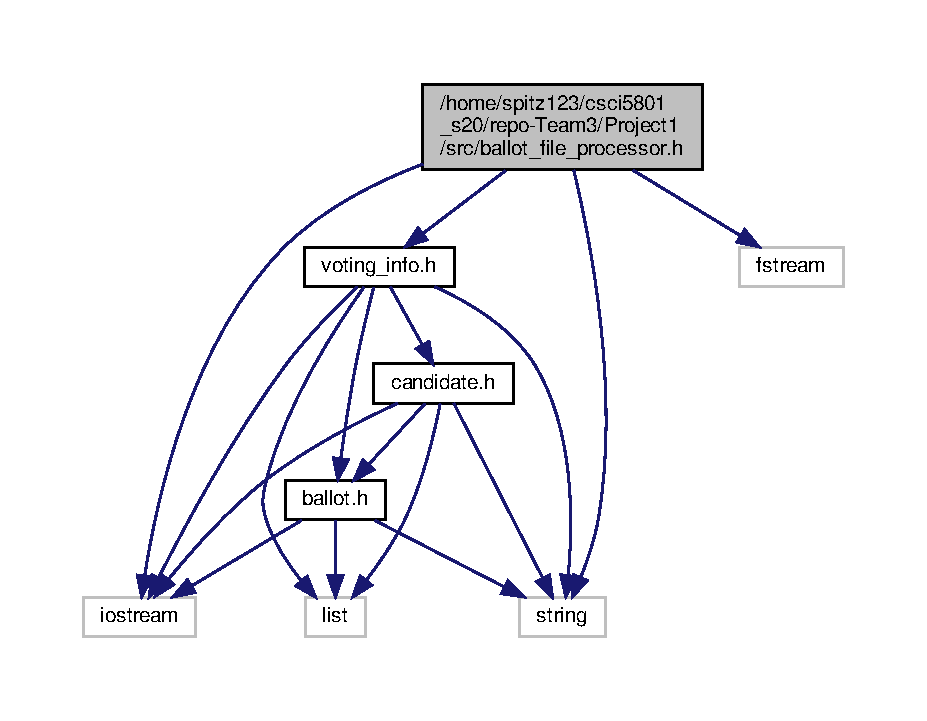
\includegraphics[width=350pt]{ballot__file__processor_8h__incl}
\end{center}
\end{figure}
This graph shows which files directly or indirectly include this file\+:\nopagebreak
\begin{figure}[H]
\begin{center}
\leavevmode
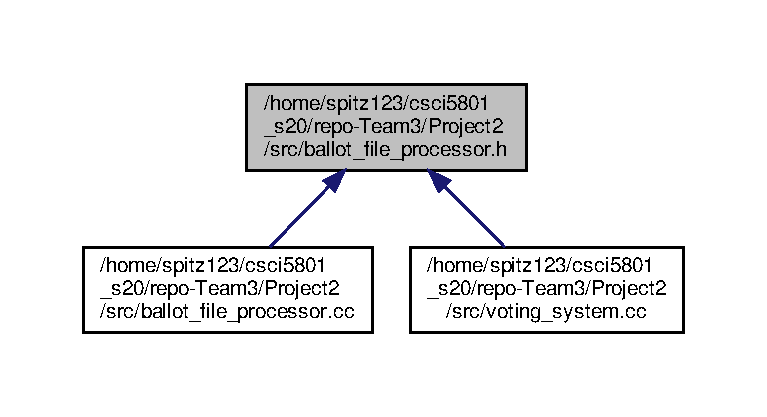
\includegraphics[width=350pt]{ballot__file__processor_8h__dep__incl}
\end{center}
\end{figure}
\subsection*{Classes}
\begin{DoxyCompactItemize}
\item 
class \hyperlink{classBallotFileProcessor}{Ballot\+File\+Processor}
\begin{DoxyCompactList}\small\item\em The main class for processing ballot files. \end{DoxyCompactList}\end{DoxyCompactItemize}
\subsection*{Variables}
\begin{DoxyCompactItemize}
\item 
\mbox{\Hypertarget{ballot__file__processor_8h_a50bd28e83c394f50c629477372b06668}\label{ballot__file__processor_8h_a50bd28e83c394f50c629477372b06668}} 
char {\bfseries Invalid\+Ballot\+File\+Name} \mbox{[}$\,$\mbox{]}
\end{DoxyCompactItemize}


\subsection{Detailed Description}
\begin{DoxyCopyright}{Copyright}
2020 Josh Spitzer-\/\+Resnick, spitz123 
\end{DoxyCopyright}

\hypertarget{candidate_8cc}{}\section{/home/spitz123/csci5801\+\_\+s20/repo-\/\+Team3/\+Project2/src/candidate.cc File Reference}
\label{candidate_8cc}\index{/home/spitz123/csci5801\+\_\+s20/repo-\/\+Team3/\+Project2/src/candidate.\+cc@{/home/spitz123/csci5801\+\_\+s20/repo-\/\+Team3/\+Project2/src/candidate.\+cc}}
{\ttfamily \#include \char`\"{}candidate.\+h\char`\"{}}\newline
{\ttfamily \#include \char`\"{}ballot.\+h\char`\"{}}\newline
Include dependency graph for candidate.\+cc\+:\nopagebreak
\begin{figure}[H]
\begin{center}
\leavevmode
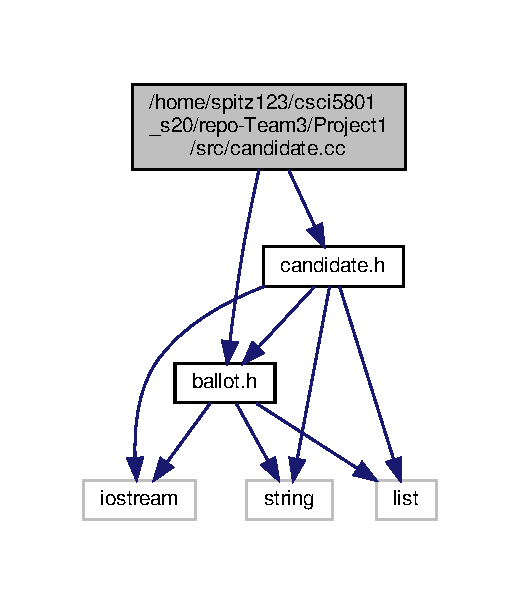
\includegraphics[width=250pt]{candidate_8cc__incl}
\end{center}
\end{figure}


\subsection{Detailed Description}
\begin{DoxyCopyright}{Copyright}
2020 5801 Team3, All rights reserved. 
\end{DoxyCopyright}

\hypertarget{candidate_8h}{}\section{/home/spitz123/csci5801\+\_\+s20/repo-\/\+Team3/\+Project1/src/candidate.h File Reference}
\label{candidate_8h}\index{/home/spitz123/csci5801\+\_\+s20/repo-\/\+Team3/\+Project1/src/candidate.\+h@{/home/spitz123/csci5801\+\_\+s20/repo-\/\+Team3/\+Project1/src/candidate.\+h}}
{\ttfamily \#include $<$iostream$>$}\newline
{\ttfamily \#include $<$string$>$}\newline
{\ttfamily \#include $<$list$>$}\newline
{\ttfamily \#include \char`\"{}ballot.\+h\char`\"{}}\newline
Include dependency graph for candidate.\+h\+:
\nopagebreak
\begin{figure}[H]
\begin{center}
\leavevmode
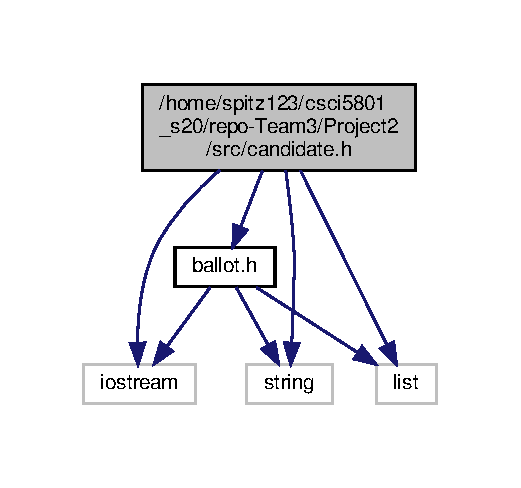
\includegraphics[width=250pt]{candidate_8h__incl}
\end{center}
\end{figure}
This graph shows which files directly or indirectly include this file\+:
\nopagebreak
\begin{figure}[H]
\begin{center}
\leavevmode
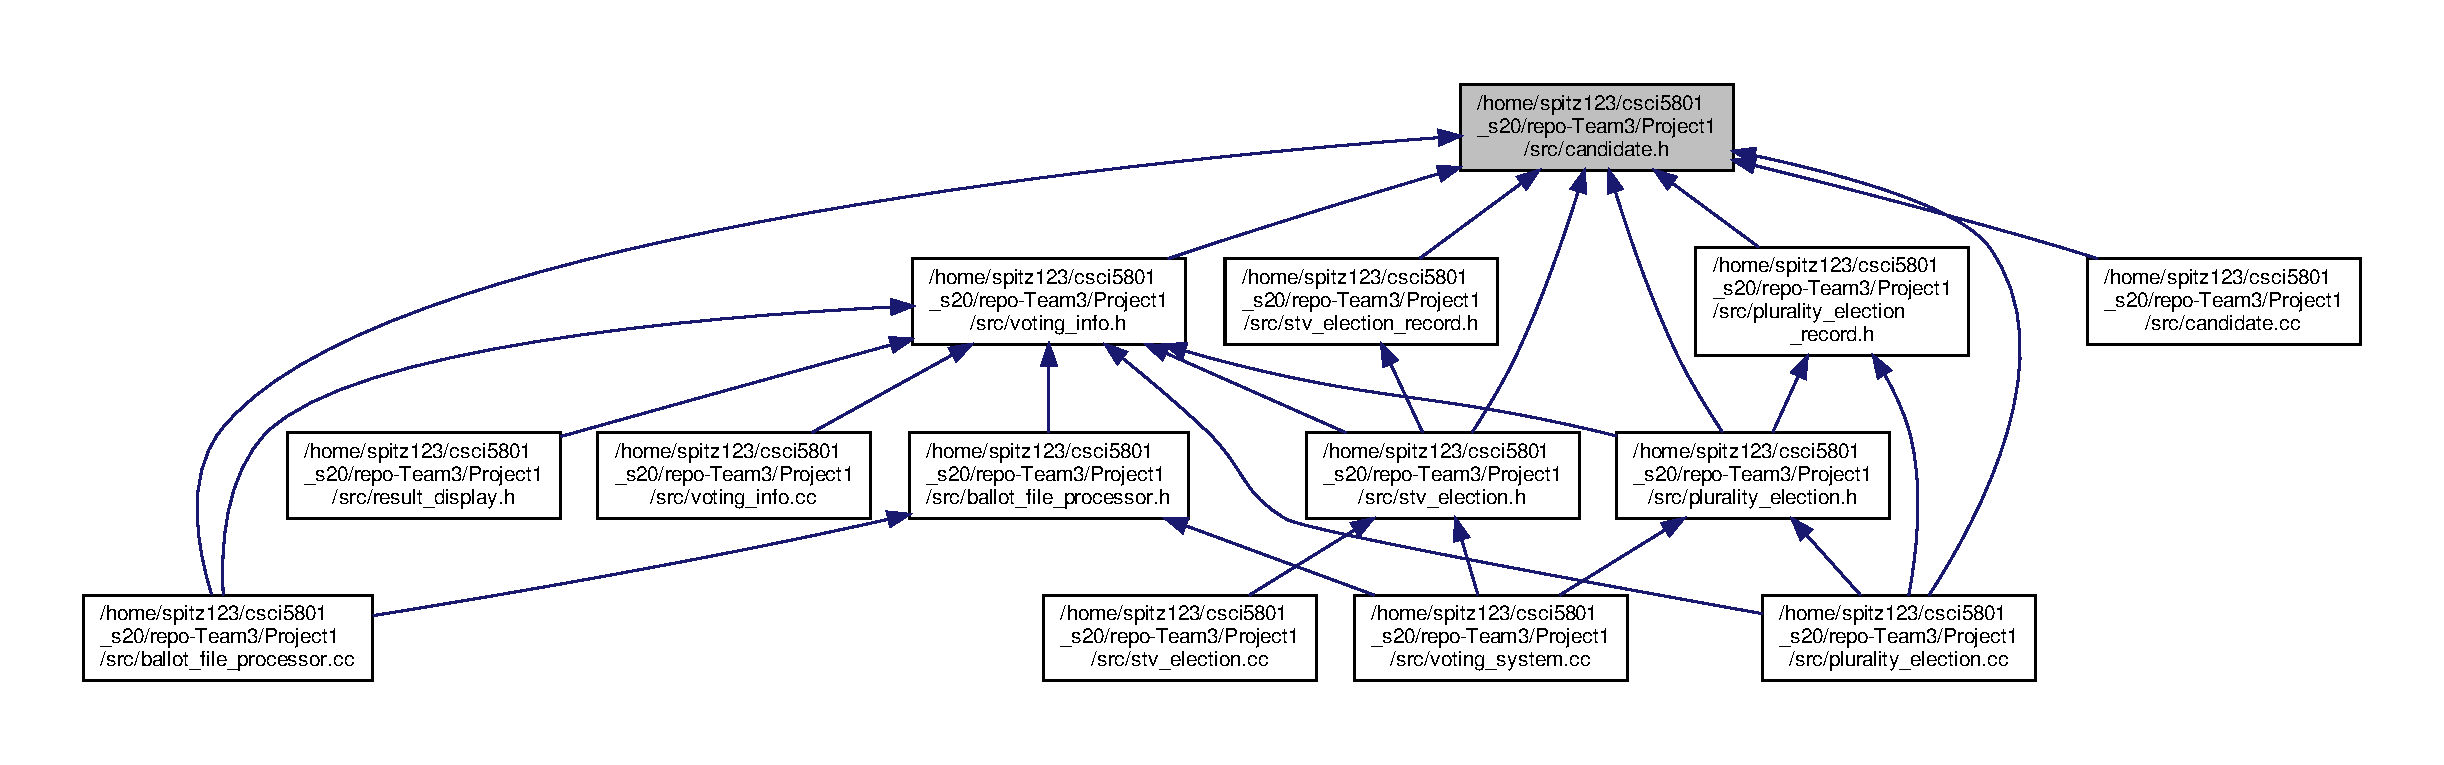
\includegraphics[width=350pt]{candidate_8h__dep__incl}
\end{center}
\end{figure}
\subsection*{Classes}
\begin{DoxyCompactItemize}
\item 
class \hyperlink{classCandidate}{Candidate}
\begin{DoxyCompactList}\small\item\em The main class for candidates. \end{DoxyCompactList}\item 
class \hyperlink{classSTVCandidate}{S\+T\+V\+Candidate}
\begin{DoxyCompactList}\small\item\em The main class for S\+TV candidates. \end{DoxyCompactList}\end{DoxyCompactItemize}


\subsection{Detailed Description}
\begin{DoxyCopyright}{Copyright}
2020 5801 Team3, All rights reserved. 
\end{DoxyCopyright}

\input{logger_8cc}
\hypertarget{logger_8h}{}\section{/home/spitz123/csci5801\+\_\+s20/repo-\/\+Team3/\+Project2/src/logger.h File Reference}
\label{logger_8h}\index{/home/spitz123/csci5801\+\_\+s20/repo-\/\+Team3/\+Project2/src/logger.\+h@{/home/spitz123/csci5801\+\_\+s20/repo-\/\+Team3/\+Project2/src/logger.\+h}}
{\ttfamily \#include $<$fstream$>$}\newline
{\ttfamily \#include $<$string$>$}\newline
{\ttfamily \#include $<$iostream$>$}\newline
{\ttfamily \#include $<$cstdlib$>$}\newline
{\ttfamily \#include $<$list$>$}\newline
{\ttfamily \#include $<$string.\+h$>$}\newline
{\ttfamily \#include \char`\"{}candidate.\+h\char`\"{}}\newline
Include dependency graph for logger.\+h\+:\nopagebreak
\begin{figure}[H]
\begin{center}
\leavevmode
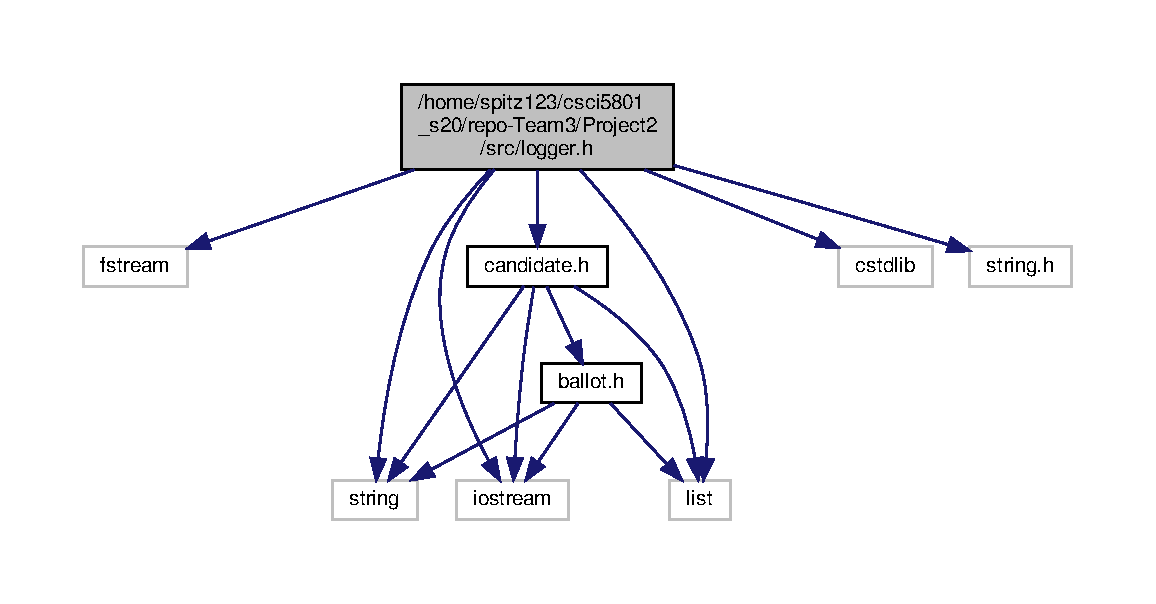
\includegraphics[width=350pt]{logger_8h__incl}
\end{center}
\end{figure}
This graph shows which files directly or indirectly include this file\+:\nopagebreak
\begin{figure}[H]
\begin{center}
\leavevmode
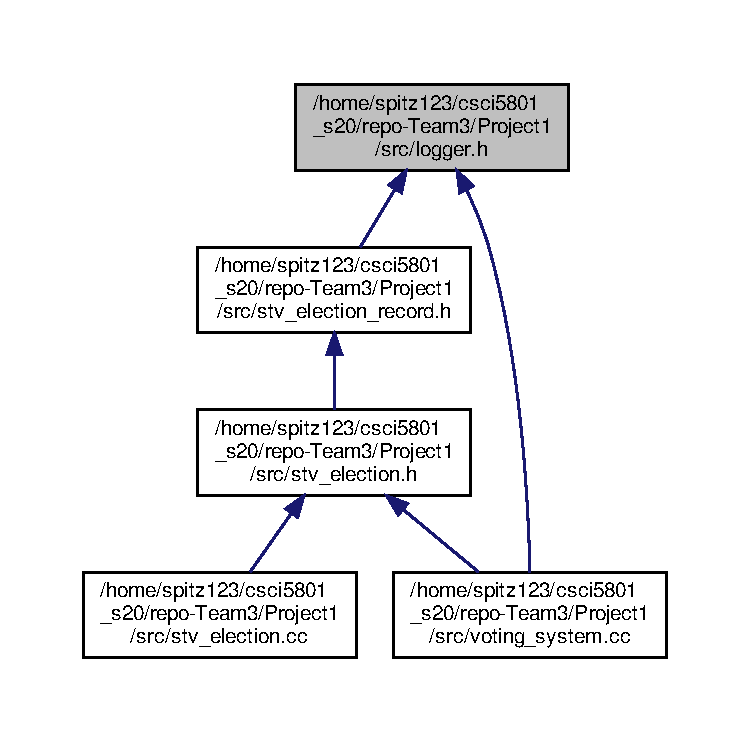
\includegraphics[width=350pt]{logger_8h__dep__incl}
\end{center}
\end{figure}
\subsection*{Classes}
\begin{DoxyCompactItemize}
\item 
class \hyperlink{classLogger}{Logger}
\begin{DoxyCompactList}\small\item\em Singleton \hyperlink{classLogger}{Logger} Class. \end{DoxyCompactList}\end{DoxyCompactItemize}
\subsection*{Macros}
\begin{DoxyCompactItemize}
\item 
\mbox{\Hypertarget{logger_8h_aa385268d3ec7b4d3ecceb7c787171bf0}\label{logger_8h_aa385268d3ec7b4d3ecceb7c787171bf0}} 
\#define {\bfseries L\+O\+G\+G\+ER}~\hyperlink{classLogger_ae85cfbef8b7e6940475a5012fa1935c6}{Logger\+::\+Get\+Logger}()
\end{DoxyCompactItemize}
\subsection*{Variables}
\begin{DoxyCompactItemize}
\item 
\mbox{\Hypertarget{logger_8h_acb3500d6229786d99850d47d1d9c6ee1}\label{logger_8h_acb3500d6229786d99850d47d1d9c6ee1}} 
char {\bfseries Log\+File\+Name} \mbox{[}$\,$\mbox{]}
\end{DoxyCompactItemize}


\subsection{Detailed Description}
\begin{DoxyCopyright}{Copyright}
2020 5801 Team3, based on a singleton logger example, All rights reserved. 
\end{DoxyCopyright}

\hypertarget{mainpage_8h}{}\section{/home/spitz123/csci5801\+\_\+s20/repo-\/\+Team3/\+Project2/src/mainpage.h File Reference}
\label{mainpage_8h}\index{/home/spitz123/csci5801\+\_\+s20/repo-\/\+Team3/\+Project2/src/mainpage.\+h@{/home/spitz123/csci5801\+\_\+s20/repo-\/\+Team3/\+Project2/src/mainpage.\+h}}


\subsection{Detailed Description}
\begin{DoxyCopyright}{Copyright}
2020 Josh Spitzer-\/\+Resnick, spitz123 
\end{DoxyCopyright}

\hypertarget{plurality__election_8cc}{}\section{/home/spitz123/csci5801\+\_\+s20/repo-\/\+Team3/\+Project1/src/plurality\+\_\+election.cc File Reference}
\label{plurality__election_8cc}\index{/home/spitz123/csci5801\+\_\+s20/repo-\/\+Team3/\+Project1/src/plurality\+\_\+election.\+cc@{/home/spitz123/csci5801\+\_\+s20/repo-\/\+Team3/\+Project1/src/plurality\+\_\+election.\+cc}}
{\ttfamily \#include \char`\"{}plurality\+\_\+election.\+h\char`\"{}}\newline
{\ttfamily \#include \char`\"{}plurality\+\_\+election\+\_\+record.\+h\char`\"{}}\newline
{\ttfamily \#include \char`\"{}voting\+\_\+info.\+h\char`\"{}}\newline
{\ttfamily \#include \char`\"{}candidate.\+h\char`\"{}}\newline
{\ttfamily \#include \char`\"{}ballot.\+h\char`\"{}}\newline
Include dependency graph for plurality\+\_\+election.\+cc\+:
\nopagebreak
\begin{figure}[H]
\begin{center}
\leavevmode
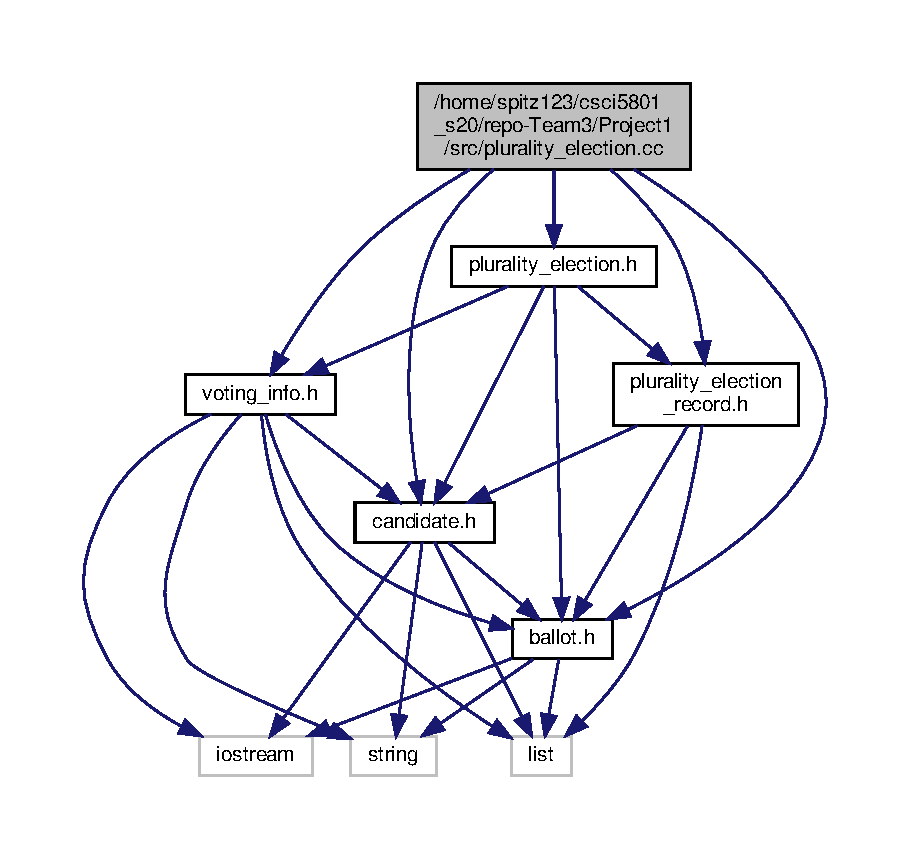
\includegraphics[width=350pt]{plurality__election_8cc__incl}
\end{center}
\end{figure}


\subsection{Detailed Description}
\begin{DoxyCopyright}{Copyright}
2020 5801 Team3, All rights reserved. 
\end{DoxyCopyright}

\hypertarget{plurality__election_8h}{}\section{/home/spitz123/csci5801\+\_\+s20/repo-\/\+Team3/\+Project1/src/plurality\+\_\+election.h File Reference}
\label{plurality__election_8h}\index{/home/spitz123/csci5801\+\_\+s20/repo-\/\+Team3/\+Project1/src/plurality\+\_\+election.\+h@{/home/spitz123/csci5801\+\_\+s20/repo-\/\+Team3/\+Project1/src/plurality\+\_\+election.\+h}}
{\ttfamily \#include \char`\"{}voting\+\_\+info.\+h\char`\"{}}\newline
{\ttfamily \#include \char`\"{}candidate.\+h\char`\"{}}\newline
{\ttfamily \#include \char`\"{}ballot.\+h\char`\"{}}\newline
{\ttfamily \#include \char`\"{}plurality\+\_\+election\+\_\+record.\+h\char`\"{}}\newline
Include dependency graph for plurality\+\_\+election.\+h\+:
\nopagebreak
\begin{figure}[H]
\begin{center}
\leavevmode
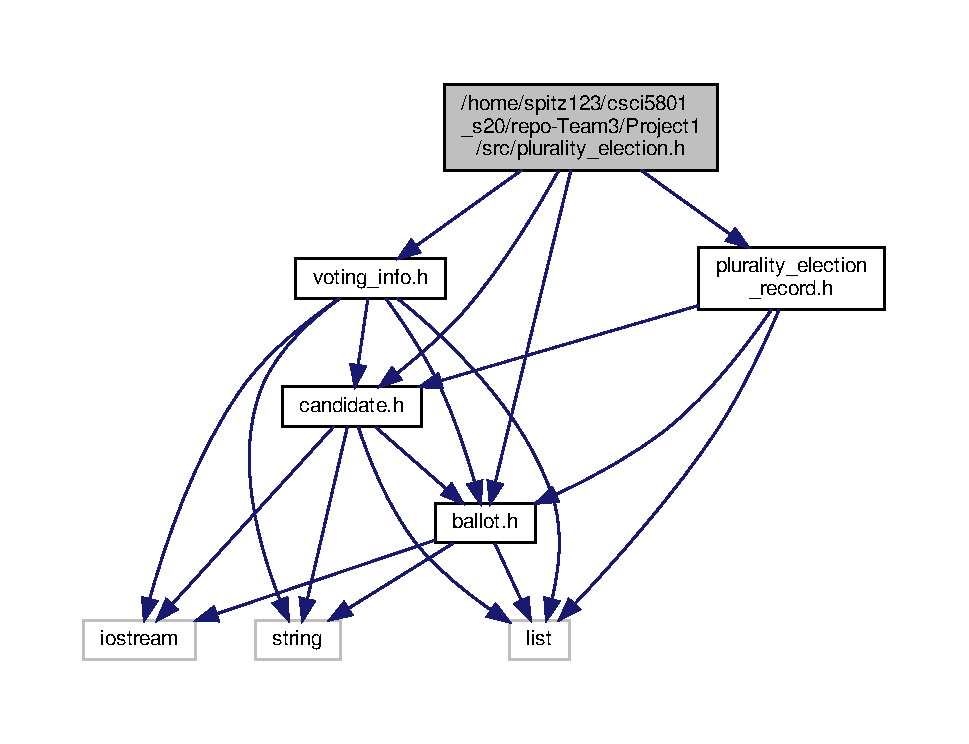
\includegraphics[width=350pt]{plurality__election_8h__incl}
\end{center}
\end{figure}
This graph shows which files directly or indirectly include this file\+:
\nopagebreak
\begin{figure}[H]
\begin{center}
\leavevmode
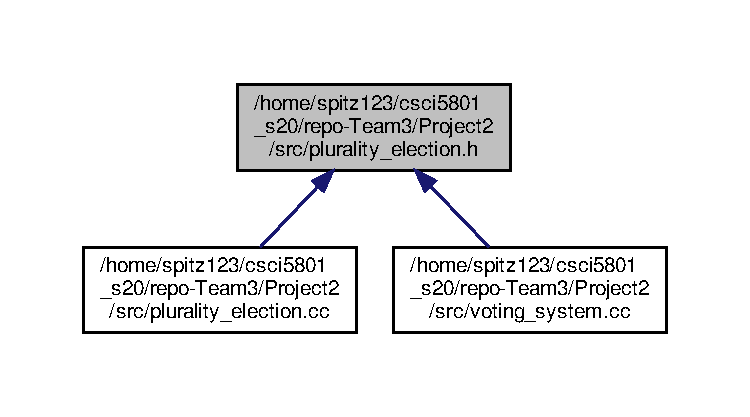
\includegraphics[width=350pt]{plurality__election_8h__dep__incl}
\end{center}
\end{figure}
\subsection*{Classes}
\begin{DoxyCompactItemize}
\item 
class \hyperlink{classPluralityElection}{Plurality\+Election}
\begin{DoxyCompactList}\small\item\em The main class for plurality election. \end{DoxyCompactList}\end{DoxyCompactItemize}


\subsection{Detailed Description}
\begin{DoxyCopyright}{Copyright}
2020 5801 Team3, All rights reserved. 
\end{DoxyCopyright}

\hypertarget{plurality__election__record_8h}{}\section{/home/spitz123/csci5801\+\_\+s20/repo-\/\+Team3/\+Project1/src/plurality\+\_\+election\+\_\+record.h File Reference}
\label{plurality__election__record_8h}\index{/home/spitz123/csci5801\+\_\+s20/repo-\/\+Team3/\+Project1/src/plurality\+\_\+election\+\_\+record.\+h@{/home/spitz123/csci5801\+\_\+s20/repo-\/\+Team3/\+Project1/src/plurality\+\_\+election\+\_\+record.\+h}}
{\ttfamily \#include $<$list$>$}\newline
{\ttfamily \#include \char`\"{}candidate.\+h\char`\"{}}\newline
{\ttfamily \#include \char`\"{}ballot.\+h\char`\"{}}\newline
Include dependency graph for plurality\+\_\+election\+\_\+record.\+h\+:
\nopagebreak
\begin{figure}[H]
\begin{center}
\leavevmode
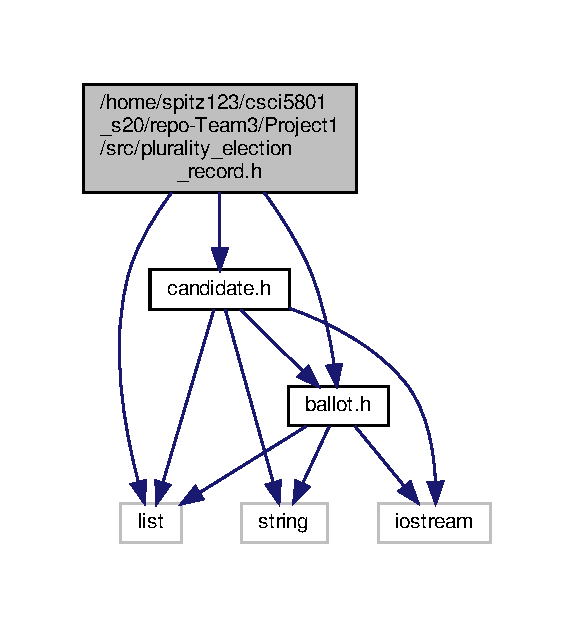
\includegraphics[width=276pt]{plurality__election__record_8h__incl}
\end{center}
\end{figure}
This graph shows which files directly or indirectly include this file\+:
\nopagebreak
\begin{figure}[H]
\begin{center}
\leavevmode
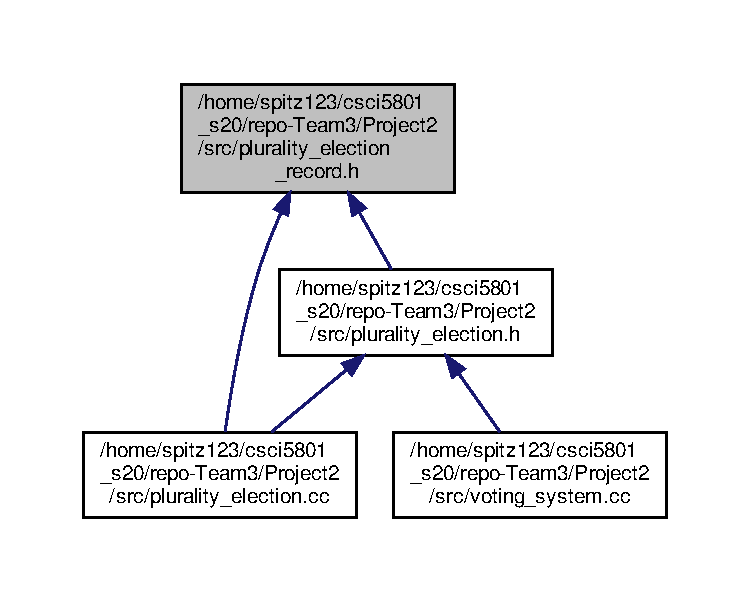
\includegraphics[width=350pt]{plurality__election__record_8h__dep__incl}
\end{center}
\end{figure}
\subsection*{Classes}
\begin{DoxyCompactItemize}
\item 
class \hyperlink{classPluralityElectionRecord}{Plurality\+Election\+Record}
\end{DoxyCompactItemize}


\subsection{Detailed Description}
\begin{DoxyCopyright}{Copyright}
2020 5801 Team3, All rights reserved. 
\end{DoxyCopyright}

\hypertarget{stv__election_8cc}{}\section{/home/spitz123/csci5801\+\_\+s20/repo-\/\+Team3/\+Project2/src/stv\+\_\+election.cc File Reference}
\label{stv__election_8cc}\index{/home/spitz123/csci5801\+\_\+s20/repo-\/\+Team3/\+Project2/src/stv\+\_\+election.\+cc@{/home/spitz123/csci5801\+\_\+s20/repo-\/\+Team3/\+Project2/src/stv\+\_\+election.\+cc}}
{\ttfamily \#include \char`\"{}stv\+\_\+election.\+h\char`\"{}}\newline
Include dependency graph for stv\+\_\+election.\+cc\+:\nopagebreak
\begin{figure}[H]
\begin{center}
\leavevmode
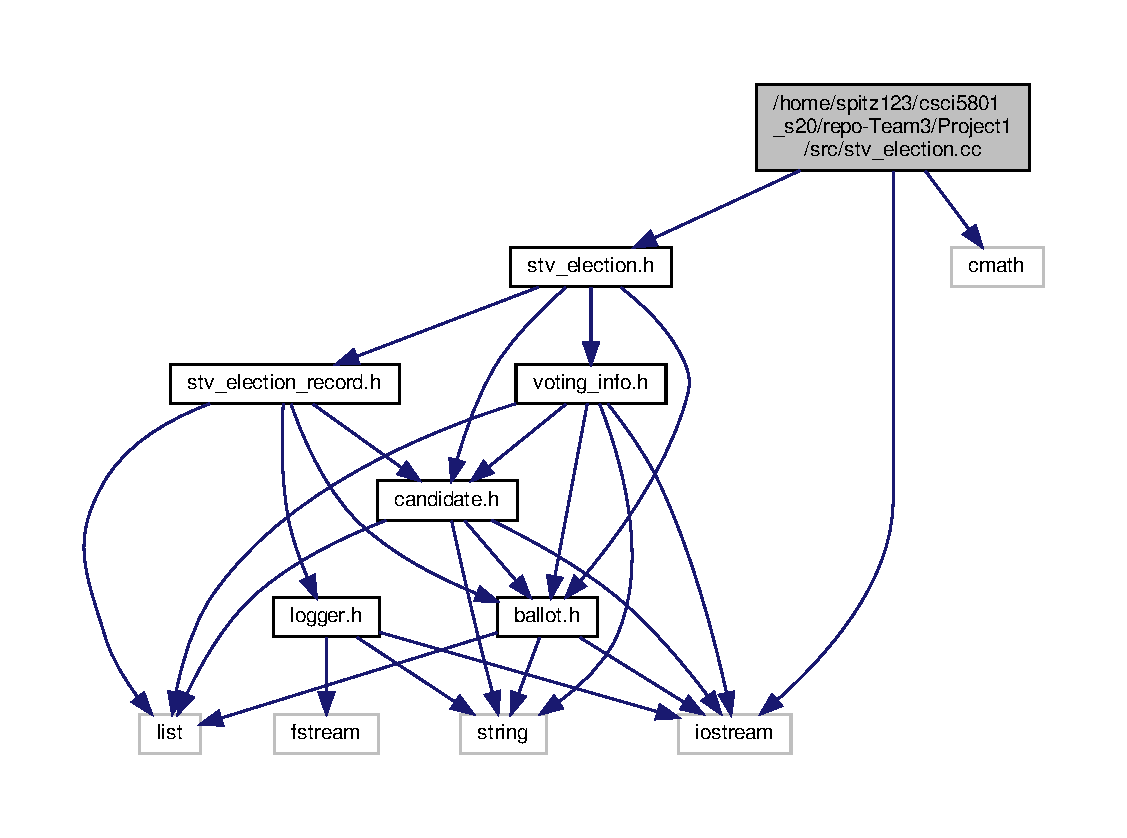
\includegraphics[width=350pt]{stv__election_8cc__incl}
\end{center}
\end{figure}


\subsection{Detailed Description}
\begin{DoxyCopyright}{Copyright}
2020 5801 Team3, All rights reserved. 
\end{DoxyCopyright}

\hypertarget{stv__election_8h}{}\section{/home/spitz123/csci5801\+\_\+s20/repo-\/\+Team3/\+Project1/src/stv\+\_\+election.h File Reference}
\label{stv__election_8h}\index{/home/spitz123/csci5801\+\_\+s20/repo-\/\+Team3/\+Project1/src/stv\+\_\+election.\+h@{/home/spitz123/csci5801\+\_\+s20/repo-\/\+Team3/\+Project1/src/stv\+\_\+election.\+h}}
{\ttfamily \#include \char`\"{}voting\+\_\+info.\+h\char`\"{}}\newline
{\ttfamily \#include \char`\"{}stv\+\_\+election\+\_\+record.\+h\char`\"{}}\newline
{\ttfamily \#include \char`\"{}candidate.\+h\char`\"{}}\newline
{\ttfamily \#include \char`\"{}ballot.\+h\char`\"{}}\newline
Include dependency graph for stv\+\_\+election.\+h\+:\nopagebreak
\begin{figure}[H]
\begin{center}
\leavevmode
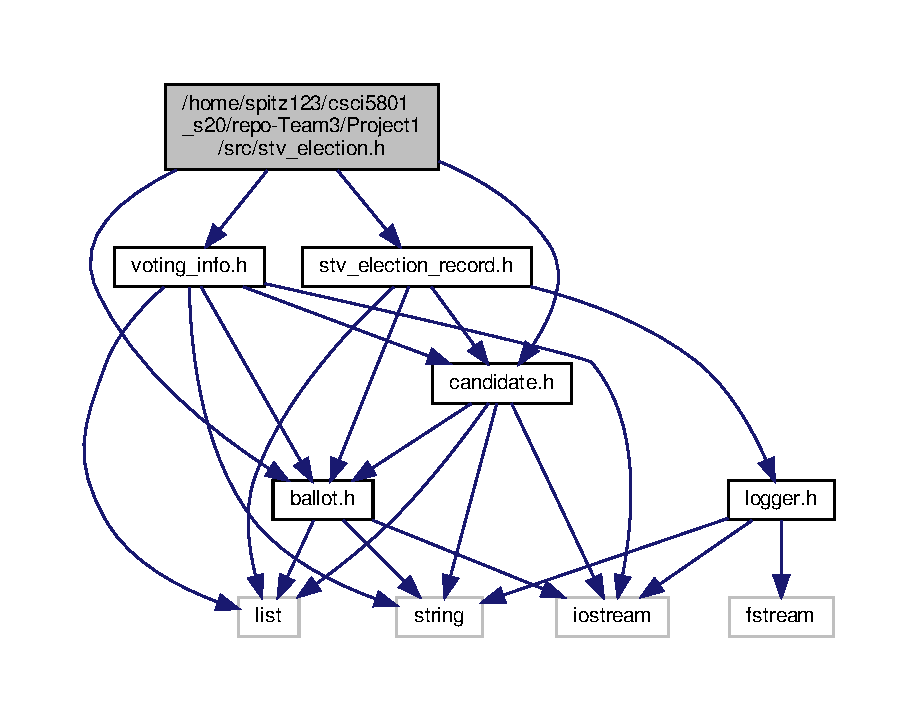
\includegraphics[width=350pt]{stv__election_8h__incl}
\end{center}
\end{figure}
This graph shows which files directly or indirectly include this file\+:\nopagebreak
\begin{figure}[H]
\begin{center}
\leavevmode
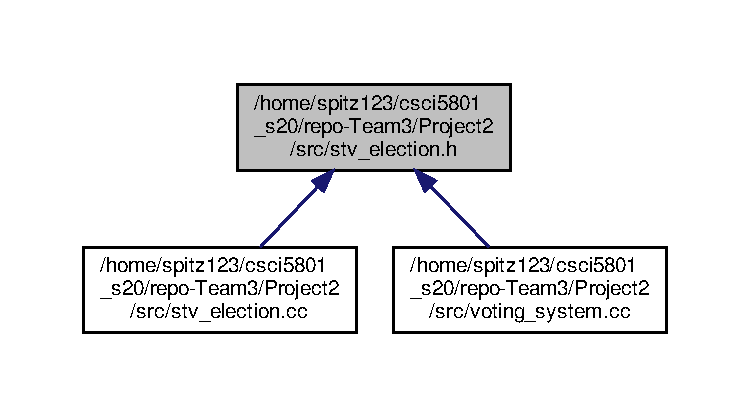
\includegraphics[width=350pt]{stv__election_8h__dep__incl}
\end{center}
\end{figure}
\subsection*{Classes}
\begin{DoxyCompactItemize}
\item 
class \hyperlink{classSTVElection}{S\+T\+V\+Election}
\begin{DoxyCompactList}\small\item\em The main class for stv election. \end{DoxyCompactList}\end{DoxyCompactItemize}
\subsection*{Variables}
\begin{DoxyCompactItemize}
\item 
\mbox{\Hypertarget{stv__election_8h_ae811c1b079da1d8b8a14de2dc5a95e12}\label{stv__election_8h_ae811c1b079da1d8b8a14de2dc5a95e12}} 
bool {\bfseries Ballot\+Shuffle\+Off}
\end{DoxyCompactItemize}


\subsection{Detailed Description}
\begin{DoxyCopyright}{Copyright}
2020 5801 Team3, All rights reserved. 
\end{DoxyCopyright}

\hypertarget{stv__election__record_8h}{}\section{/home/spitz123/csci5801\+\_\+s20/repo-\/\+Team3/\+Project1/src/stv\+\_\+election\+\_\+record.h File Reference}
\label{stv__election__record_8h}\index{/home/spitz123/csci5801\+\_\+s20/repo-\/\+Team3/\+Project1/src/stv\+\_\+election\+\_\+record.\+h@{/home/spitz123/csci5801\+\_\+s20/repo-\/\+Team3/\+Project1/src/stv\+\_\+election\+\_\+record.\+h}}
{\ttfamily \#include $<$list$>$}\newline
{\ttfamily \#include \char`\"{}candidate.\+h\char`\"{}}\newline
{\ttfamily \#include \char`\"{}ballot.\+h\char`\"{}}\newline
{\ttfamily \#include \char`\"{}logger.\+h\char`\"{}}\newline
Include dependency graph for stv\+\_\+election\+\_\+record.\+h\+:
\nopagebreak
\begin{figure}[H]
\begin{center}
\leavevmode
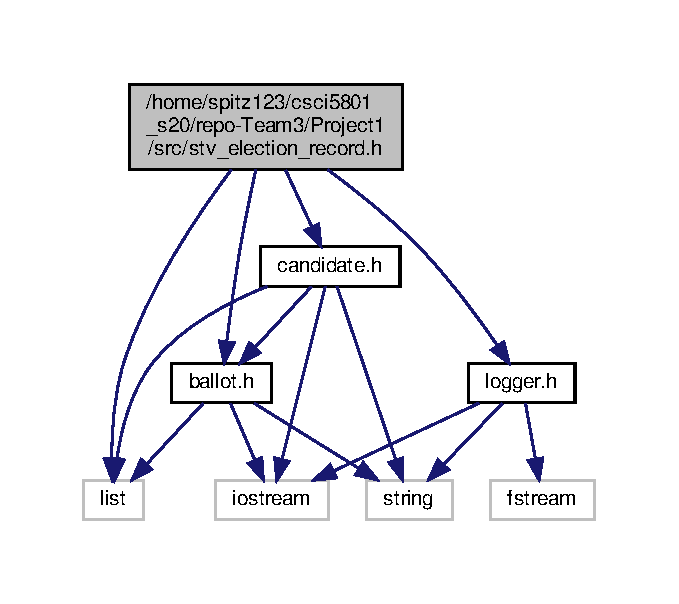
\includegraphics[width=326pt]{stv__election__record_8h__incl}
\end{center}
\end{figure}
This graph shows which files directly or indirectly include this file\+:
\nopagebreak
\begin{figure}[H]
\begin{center}
\leavevmode
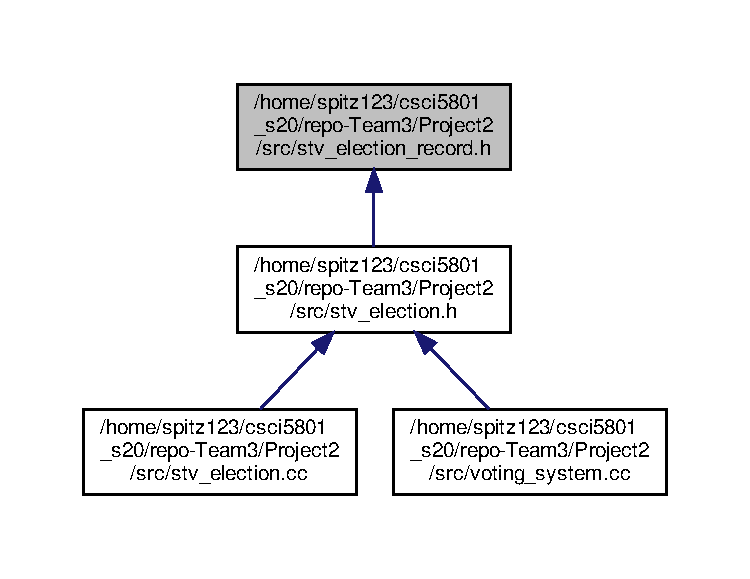
\includegraphics[width=350pt]{stv__election__record_8h__dep__incl}
\end{center}
\end{figure}
\subsection*{Classes}
\begin{DoxyCompactItemize}
\item 
class \hyperlink{classSTVElectionRecord}{S\+T\+V\+Election\+Record}
\begin{DoxyCompactList}\small\item\em The class for the S\+TV election records. \end{DoxyCompactList}\end{DoxyCompactItemize}
\subsection*{Variables}
\begin{DoxyCompactItemize}
\item 
\mbox{\Hypertarget{stv__election__record_8h_a0009c186c3629201f6c24eded36605f4}\label{stv__election__record_8h_a0009c186c3629201f6c24eded36605f4}} 
\hyperlink{classLogger}{Logger} $\ast$ {\bfseries logger}
\end{DoxyCompactItemize}


\subsection{Detailed Description}
\begin{DoxyCopyright}{Copyright}
2020 5801 Team3, All rights reserved. 
\end{DoxyCopyright}

\hypertarget{voting__info_8cc}{}\section{/home/spitz123/csci5801\+\_\+s20/repo-\/\+Team3/\+Project1/src/voting\+\_\+info.cc File Reference}
\label{voting__info_8cc}\index{/home/spitz123/csci5801\+\_\+s20/repo-\/\+Team3/\+Project1/src/voting\+\_\+info.\+cc@{/home/spitz123/csci5801\+\_\+s20/repo-\/\+Team3/\+Project1/src/voting\+\_\+info.\+cc}}
{\ttfamily \#include $<$iostream$>$}\newline
{\ttfamily \#include $<$string$>$}\newline
{\ttfamily \#include $<$list$>$}\newline
{\ttfamily \#include \char`\"{}voting\+\_\+info.\+h\char`\"{}}\newline
Include dependency graph for voting\+\_\+info.\+cc\+:\nopagebreak
\begin{figure}[H]
\begin{center}
\leavevmode
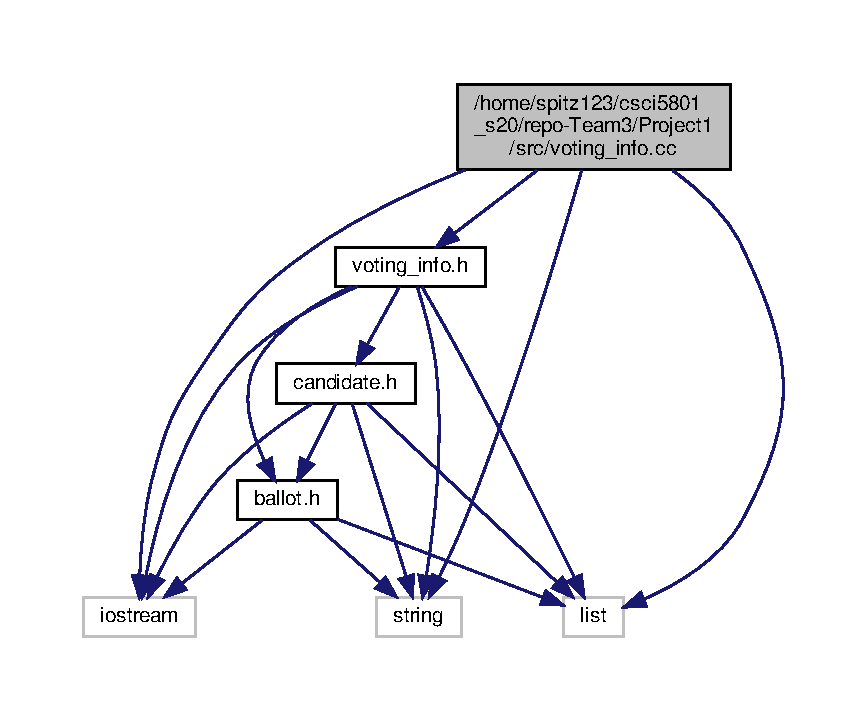
\includegraphics[width=350pt]{voting__info_8cc__incl}
\end{center}
\end{figure}


\subsection{Detailed Description}
\begin{DoxyCopyright}{Copyright}
2020 Josh Spitzer-\/\+Resnick, spitz123 
\end{DoxyCopyright}

\hypertarget{voting__info_8h}{}\section{/home/spitz123/csci5801\+\_\+s20/repo-\/\+Team3/\+Project2/src/voting\+\_\+info.h File Reference}
\label{voting__info_8h}\index{/home/spitz123/csci5801\+\_\+s20/repo-\/\+Team3/\+Project2/src/voting\+\_\+info.\+h@{/home/spitz123/csci5801\+\_\+s20/repo-\/\+Team3/\+Project2/src/voting\+\_\+info.\+h}}
{\ttfamily \#include $<$iostream$>$}\newline
{\ttfamily \#include $<$string$>$}\newline
{\ttfamily \#include $<$list$>$}\newline
{\ttfamily \#include \char`\"{}candidate.\+h\char`\"{}}\newline
{\ttfamily \#include \char`\"{}ballot.\+h\char`\"{}}\newline
Include dependency graph for voting\+\_\+info.\+h\+:\nopagebreak
\begin{figure}[H]
\begin{center}
\leavevmode
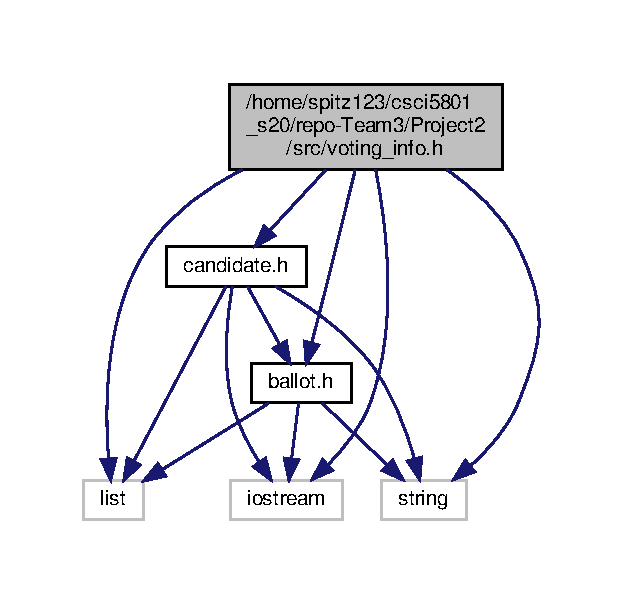
\includegraphics[width=299pt]{voting__info_8h__incl}
\end{center}
\end{figure}
This graph shows which files directly or indirectly include this file\+:\nopagebreak
\begin{figure}[H]
\begin{center}
\leavevmode
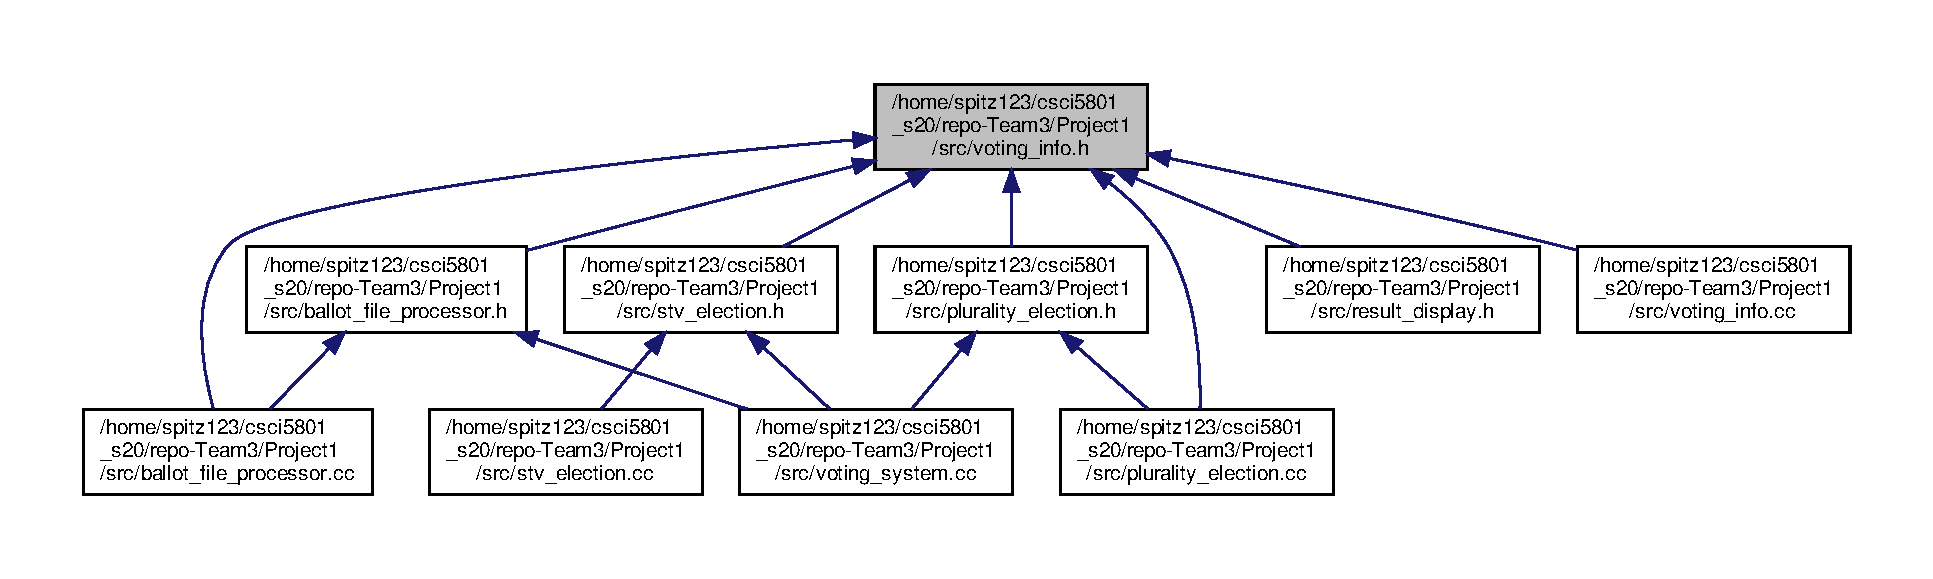
\includegraphics[width=350pt]{voting__info_8h__dep__incl}
\end{center}
\end{figure}
\subsection*{Classes}
\begin{DoxyCompactItemize}
\item 
class \hyperlink{classVotingInfo}{Voting\+Info}
\begin{DoxyCompactList}\small\item\em The main class for storing voting information. \end{DoxyCompactList}\end{DoxyCompactItemize}


\subsection{Detailed Description}
\begin{DoxyCopyright}{Copyright}
2020 5801 Team3, all rights reserved 
\end{DoxyCopyright}

\hypertarget{voting__system_8cc}{}\section{/home/spitz123/csci5801\+\_\+s20/repo-\/\+Team3/\+Project1/src/voting\+\_\+system.cc File Reference}
\label{voting__system_8cc}\index{/home/spitz123/csci5801\+\_\+s20/repo-\/\+Team3/\+Project1/src/voting\+\_\+system.\+cc@{/home/spitz123/csci5801\+\_\+s20/repo-\/\+Team3/\+Project1/src/voting\+\_\+system.\+cc}}
{\ttfamily \#include \char`\"{}stv\+\_\+election.\+h\char`\"{}}\newline
{\ttfamily \#include \char`\"{}plurality\+\_\+election.\+h\char`\"{}}\newline
{\ttfamily \#include \char`\"{}ballot\+\_\+file\+\_\+processor.\+h\char`\"{}}\newline
{\ttfamily \#include \char`\"{}logger.\+h\char`\"{}}\newline
{\ttfamily \#include $<$cstring$>$}\newline
{\ttfamily \#include $<$iostream$>$}\newline
Include dependency graph for voting\+\_\+system.\+cc\+:
\nopagebreak
\begin{figure}[H]
\begin{center}
\leavevmode
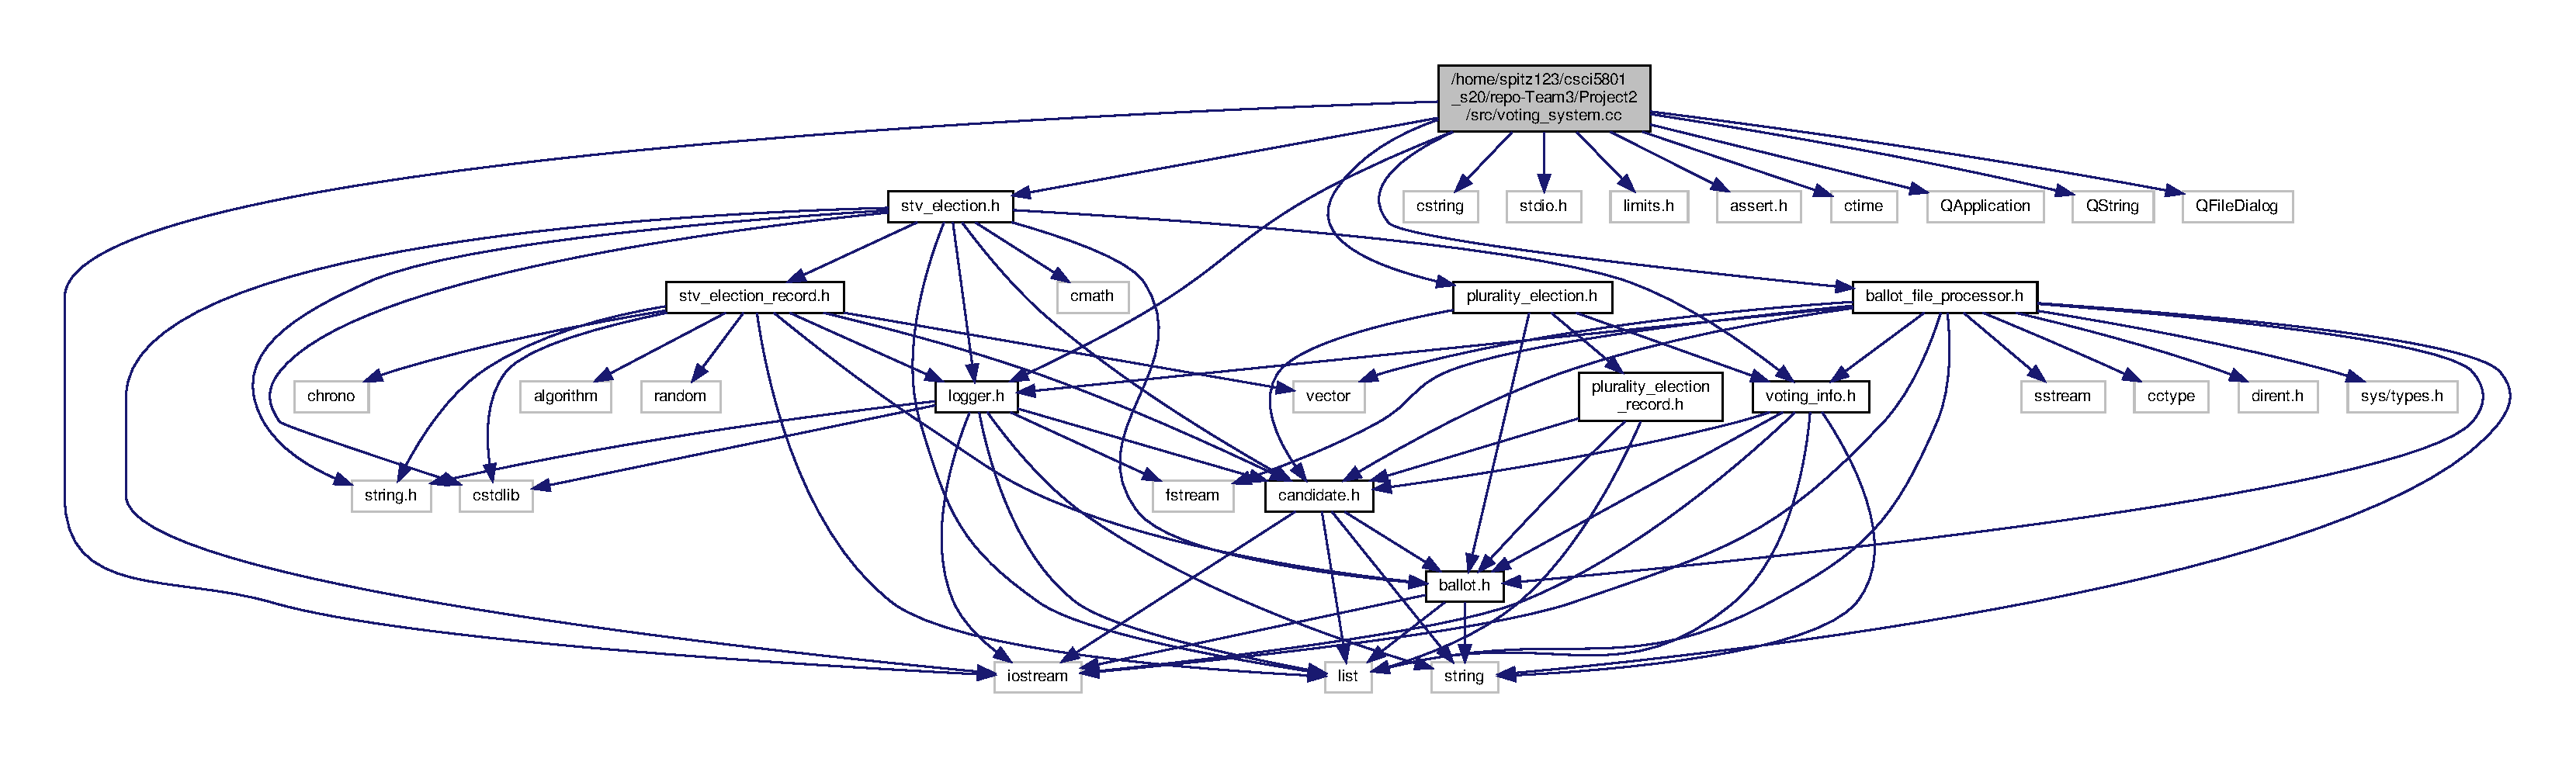
\includegraphics[width=350pt]{voting__system_8cc__incl}
\end{center}
\end{figure}
\subsection*{Functions}
\begin{DoxyCompactItemize}
\item 
\mbox{\Hypertarget{voting__system_8cc_adea641fb0c9612320d13079a7b90f346}\label{voting__system_8cc_adea641fb0c9612320d13079a7b90f346}} 
void {\bfseries User\+Interface} (int $\ast$num\+Seats, int $\ast$choice)
\item 
\mbox{\Hypertarget{voting__system_8cc_a746bd5f171a4854e01b931f9e4839876}\label{voting__system_8cc_a746bd5f171a4854e01b931f9e4839876}} 
void {\bfseries Display\+Help} ()
\item 
\mbox{\Hypertarget{voting__system_8cc_a3c04138a5bfe5d72780bb7e82a18e627}\label{voting__system_8cc_a3c04138a5bfe5d72780bb7e82a18e627}} 
int {\bfseries main} (int argc, char $\ast$$\ast$argv)
\end{DoxyCompactItemize}
\subsection*{Variables}
\begin{DoxyCompactItemize}
\item 
\mbox{\Hypertarget{voting__system_8cc_ae811c1b079da1d8b8a14de2dc5a95e12}\label{voting__system_8cc_ae811c1b079da1d8b8a14de2dc5a95e12}} 
bool {\bfseries Ballot\+Shuffle\+Off} = false
\item 
\mbox{\Hypertarget{voting__system_8cc_a0009c186c3629201f6c24eded36605f4}\label{voting__system_8cc_a0009c186c3629201f6c24eded36605f4}} 
\hyperlink{classLogger}{Logger} $\ast$ {\bfseries logger} = new \hyperlink{classLogger}{Logger}()
\end{DoxyCompactItemize}


\subsection{Detailed Description}
\begin{DoxyCopyright}{Copyright}
2020 5801 Team3, All rights reserved. 
\end{DoxyCopyright}

%--- End generated contents ---

% Index
\backmatter
\newpage
\phantomsection
\clearemptydoublepage
\addcontentsline{toc}{chapter}{Index}
\printindex

\end{document}
